\documentclass[../PianoProgetto.tex]{subfiles}
\begin{document}
	\section{Preventivo}
		\subsection{Dettaglio fasi}
			\subsubsection{Fase A}
				\paragraph{Suddivisione del lavoro}
						
	\begin{table}[h]
		%\centering
		\begin{tabularx}{\textwidth}{l  * {6}{C}  c}
			\toprule
			\textbf{Nominativo} & \textbf{Rp} & \textbf{Am} & \textbf{Pt} 
						& \textbf{An} & \textbf{Pm} & \textbf{Ve} & \textbf{Ore totali} \\
			\midrule
			Andrighetto Cristian & 0 & 15 &	0 &	10 & 0 & 15 & 40 \\
			%\midrule
			Bicego Eduard & 4 & 10 & 0 & 0 & 0 & 26 & 40 \\
			%\midrule
			Castello Davide &	0 &	20 &	0 &	10 & 0 &	10 & 40 \\
			%\midrule
			Conti Oscar Elia & 0 & 20 &	0 &	15 & 0 & 5 & 40 \\
			%\midrule
			Tavella Federico &	17 & 2 & 0 & 21 & 0 & 0 & 40 \\
			%\midrule
			Tombolato Andrea & 12 & 5 &	0 &	20 & 0 & 3 & 40 \\
			%\midrule
			Zanella Marco & 0 & 15 & 0 & 10 & 0 & 15 & 40 \\
			\midrule			
			\textbf{Ore Totali Ruolo} & 33 & 87 & 0 & 86 &	0 &	74 & 280 \\
			\bottomrule
		\end{tabularx}
		\caption{Fase A - Suddivisione delle ore di lavoro}
		\label{tab:faseA_ore}
	\end{table}

\vfill
	
	\begin{figure}[!h]
		\centering
		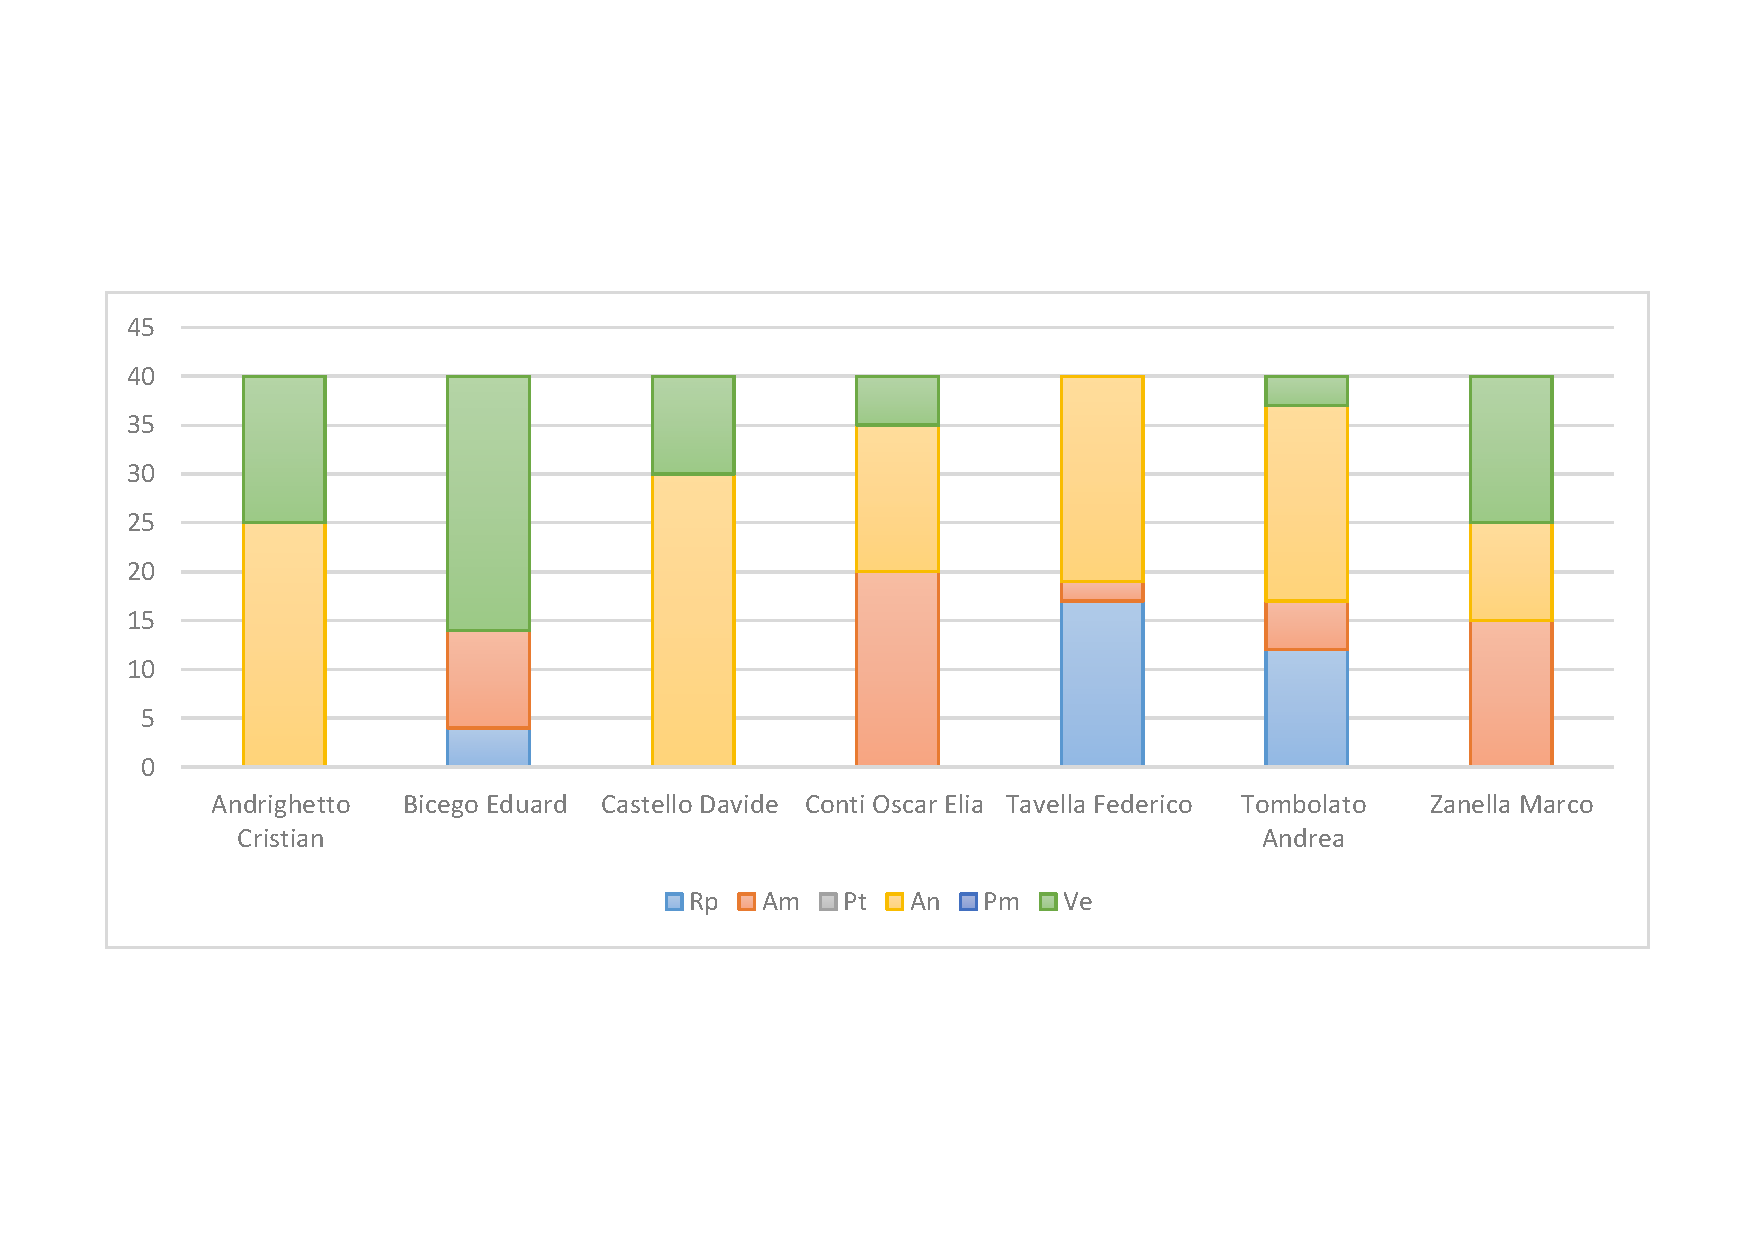
\includegraphics[width=\textwidth , trim=2cm 5cm 2cm 5cm]{grafici/A/A-ore-persona}
			\caption{Fase A - Riassunto}
		\label{fig:BarChart-faseA_ore}
	\end{figure}	
	
\newpage
	\vfill	
	\paragraph{Prospetto economico}
						
	\begin{table}[h]
		\centering
		\begin{tabular}{l * {2}{c}}
			\toprule
			\textbf{Ruolo} & \textbf{Ore} & \textbf{Costo (\euro{})} \\
			\midrule
			Responsabile &	33 &  990,00 \\
			%\midrule
			Amministratore & 87 &  1.740,00 \\
			%\midrule
			Progettista & 0 & 0,00 \\
			%\midrule
			Analista & 86 & 2,150,00 \\
			%\midrule
			Programmatore & 0 & 0,00 \\
			%\midrule
			Verificatore & 74 & 1.110,00 \\
			\midrule		
			\textbf{Totale} & 280 & 5.990,00 \\
			\bottomrule	
		\end{tabular}
		\caption{Fase A - Costo per ruolo}
		\label{tab:faseA_costo}
	\end{table}

\vfill	
	\begin{figure}[!h]
		\centering
		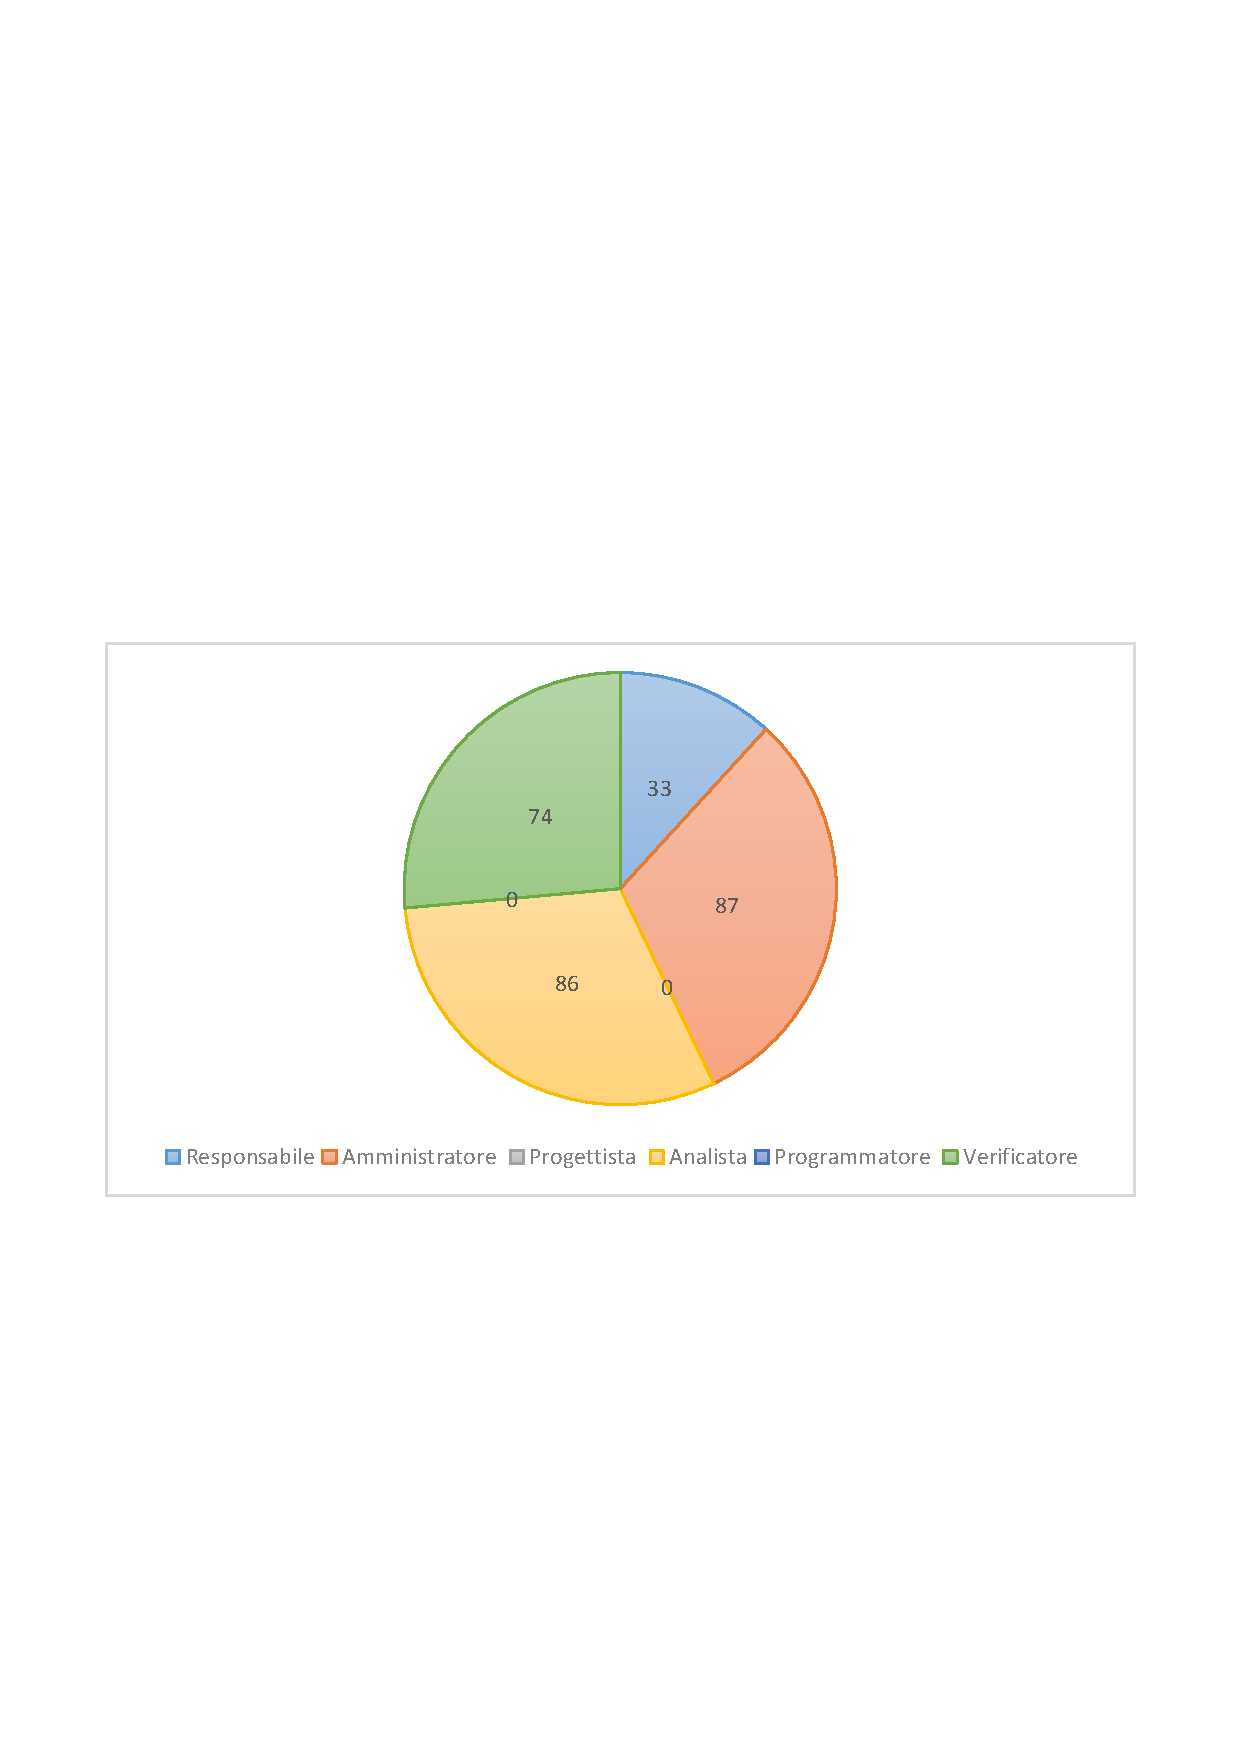
\includegraphics[width=0.93\textwidth , trim=2cm 9.5cm 2cm 11cm]{grafici/A/A-ore-ruolo}
			\caption{Fase A - Ore per ruolo}
		\label{fig:CircleChart-faseA_ore_r}
	\end{figure}
\vfill	
\newpage
\vfill	

	\begin{figure}[!h]
		\centering
		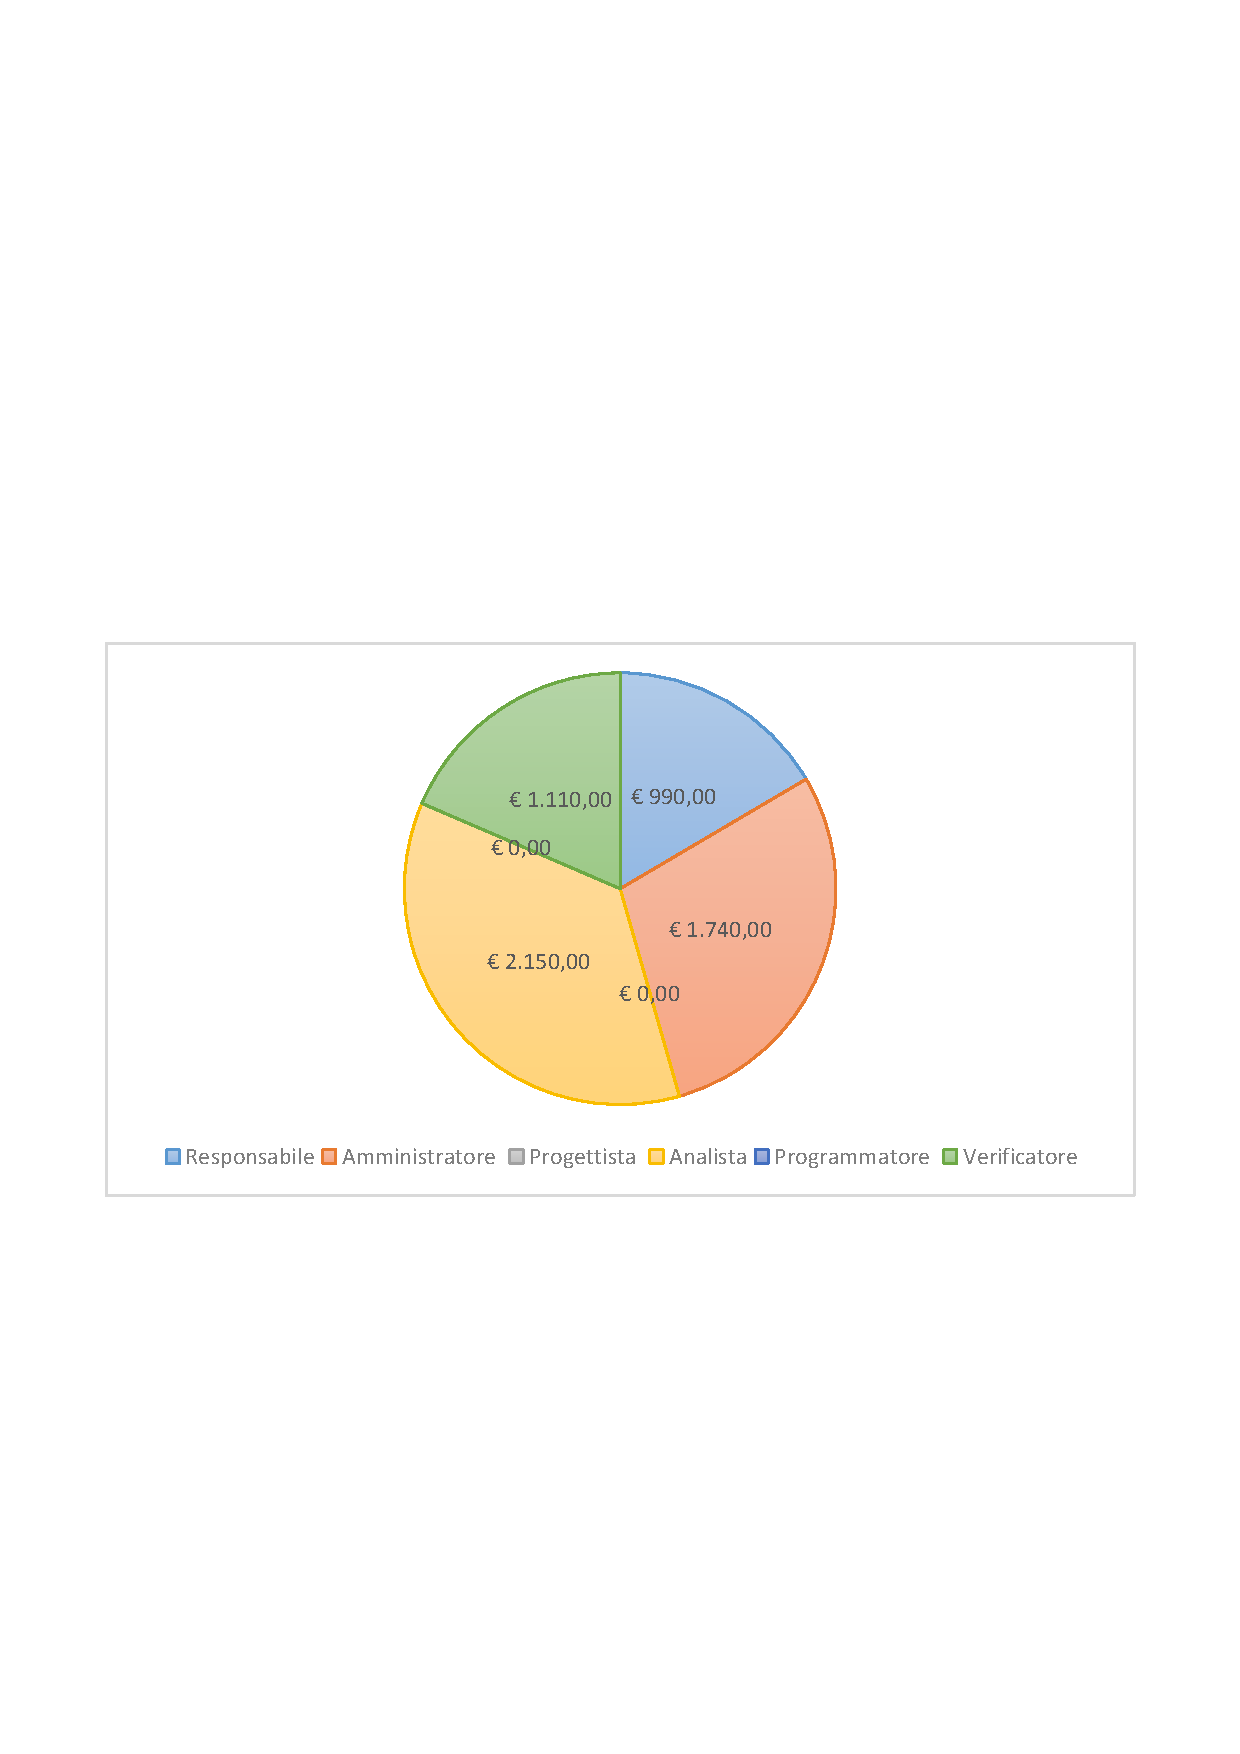
\includegraphics[width=0.93\textwidth , trim=2cm 9.5cm 2cm 11cm]{grafici/A/A-costo}
			\caption{Fase A - Costo per ruolo}
		\label{fig:CircleChart-faseA_costo}
	\end{figure}
\vfill
	
	\subsubsection{Fase AD}
				\paragraph{Suddivisione del lavoro}
				
	\begin{table}[h]
		%\centering
		\begin{tabularx}{\textwidth}{l  * {6}{C}  c}
			\toprule
			\textbf{Nominativo} & \textbf{Rp} & \textbf{Am} & \textbf{Pt} 
						& \textbf{An} & \textbf{Pm} & \textbf{Ve} & \textbf{Ore totali} \\
			\midrule
			Andrighetto Cristian & 9 & 3 &	0 &	0 & 0 & 0 & 12 \\
			%\midrule
			Bicego Eduard & 0 & 5 & 0 & 0 & 0 & 6 & 11 \\
			%\midrule
			Castello Davide & 0 & 5 & 0 & 0 & 0 & 6 & 11 \\
			%\midrule
			Conti Oscar Elia & 0 & 0 &	0 &	4 & 0 & 8 & 12 \\
			%\midrule
			Tavella Federico &	0 & 0 & 0 & 5 & 0 & 7 & 12 \\
			%\midrule
			Tombolato Andrea & 0 & 0 &	0 &	4 & 0 & 7 & 11 \\
			%\midrule
			Zanella Marco & 0 & 0 & 0 & 5 & 0 & 6 & 11 \\
			\midrule			
			\textbf{Ore Totali Ruolo} & 9 & 13 & 0 & 18 & 0 & 40 & 80 \\
			\bottomrule
		\end{tabularx}	
		\caption{Fase AD - Suddivisione delle ore di lavoro}
		\label{tab:faseAD_ore}	
	\end{table}
\vfill
\newpage
\vfill
	
	\begin{figure}[!h]
		\centering
		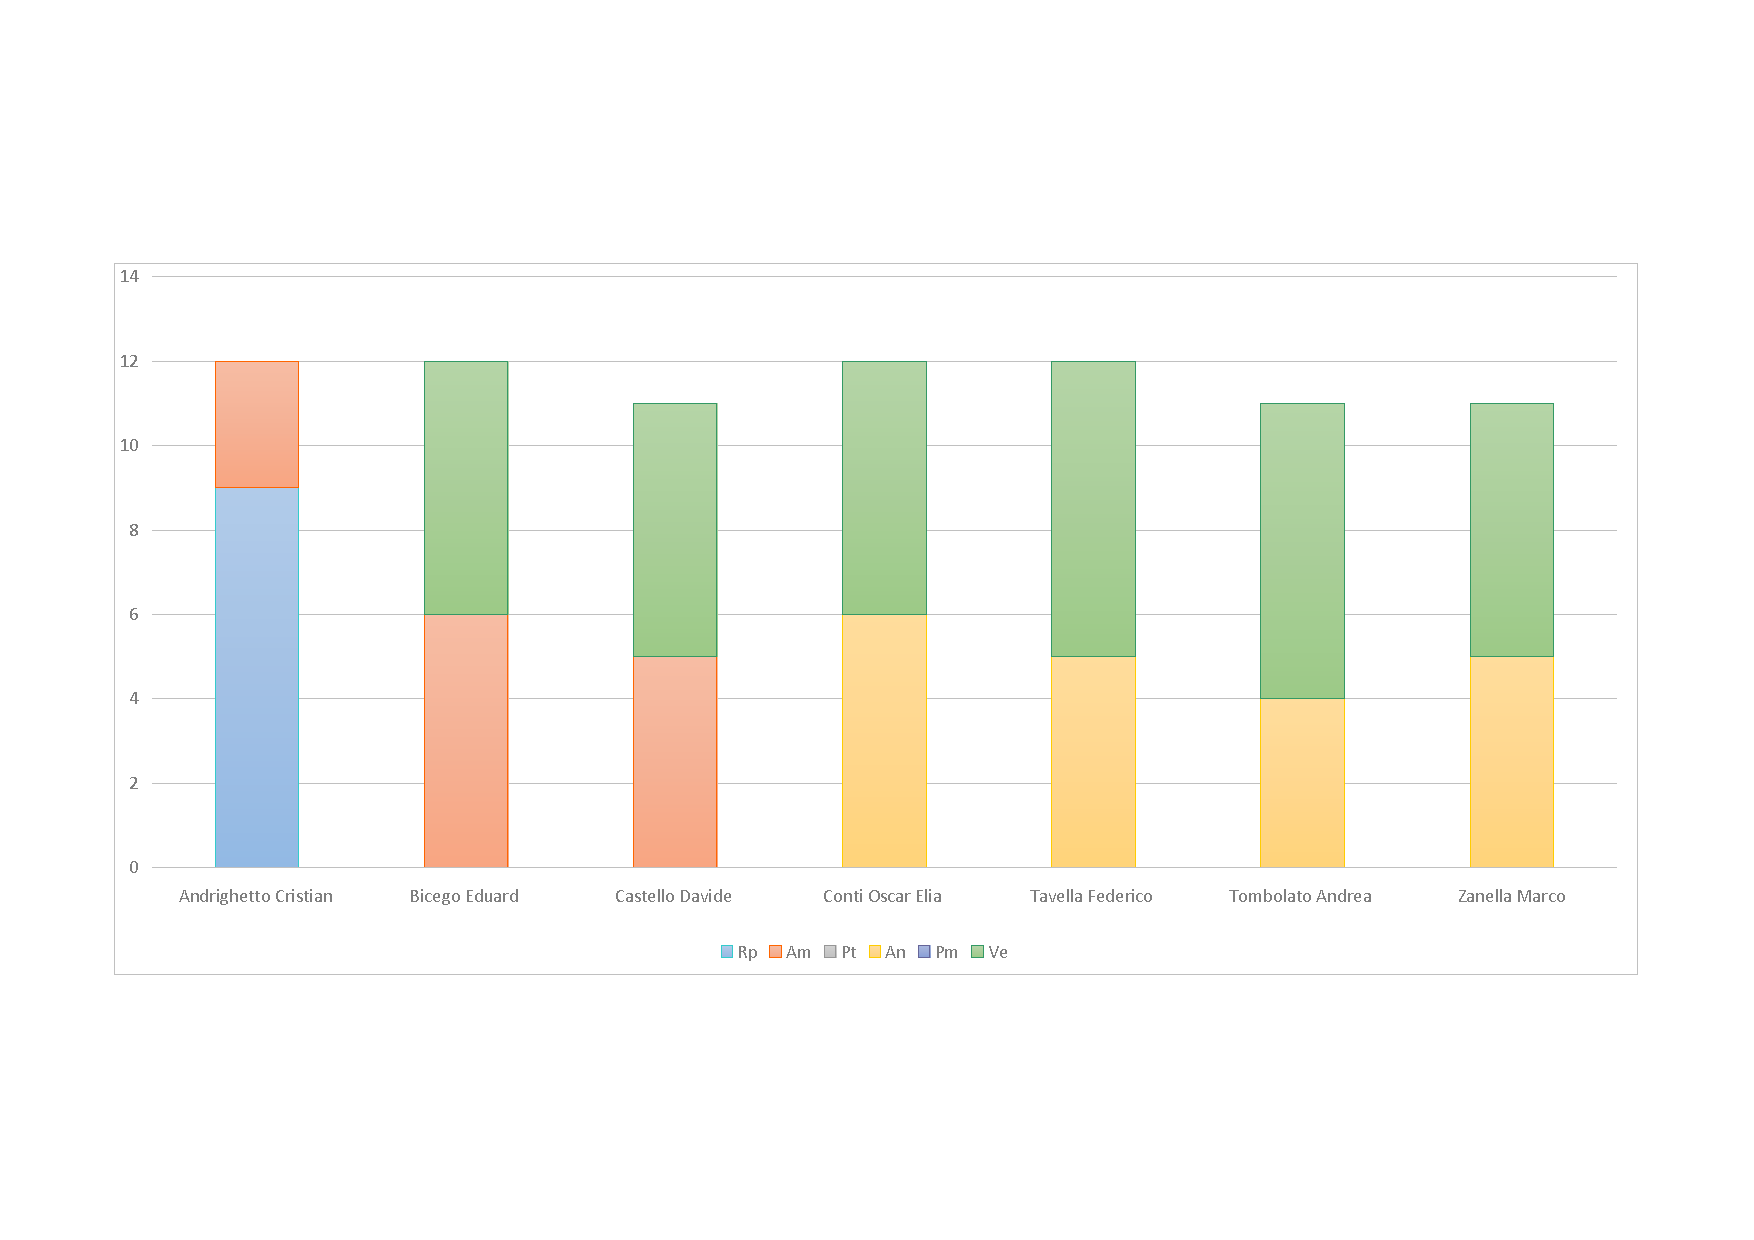
\includegraphics[width=\textwidth , trim=2cm 5cm 2cm 5cm]{grafici/AD/AD-ore-persona}
			\caption{Fase AD - Riassunto}
		\label{fig:BarChart-faseAD_ore}
	\end{figure}
	
\vfill
	
	\paragraph{Prospetto economico}
	
					\begin{table}[h]
		\centering
	
		\begin{tabular}{l * {2}{c}}
			\toprule
			\textbf{Ruolo} & \textbf{Ore} & \textbf{Costo (\euro{})} \\
			\midrule
			Responsabile &	9 & 270,00 \\
			%\midrule
			Amministratore & 13 & 260,00 \\
			%\midrule
			Progettista & 0 & 0,00 \\
			%\midrule
			Analista & 18 & 450,00 \\
			%\midrule
			Programmatore & 0 & 0,00 \\
			%\midrule
			Verificatore & 40 & 600,00 \\
			\midrule		
			\textbf{Totale} & 80 & 1.580,00 \\
			\bottomrule
		\end{tabular}
		\caption{Fase AD - Costo per ruolo}
		\label{tab:faseAD_costo}
	\end{table}
\vfill
\newpage
	
	\begin{figure}[!h]
		\centering
		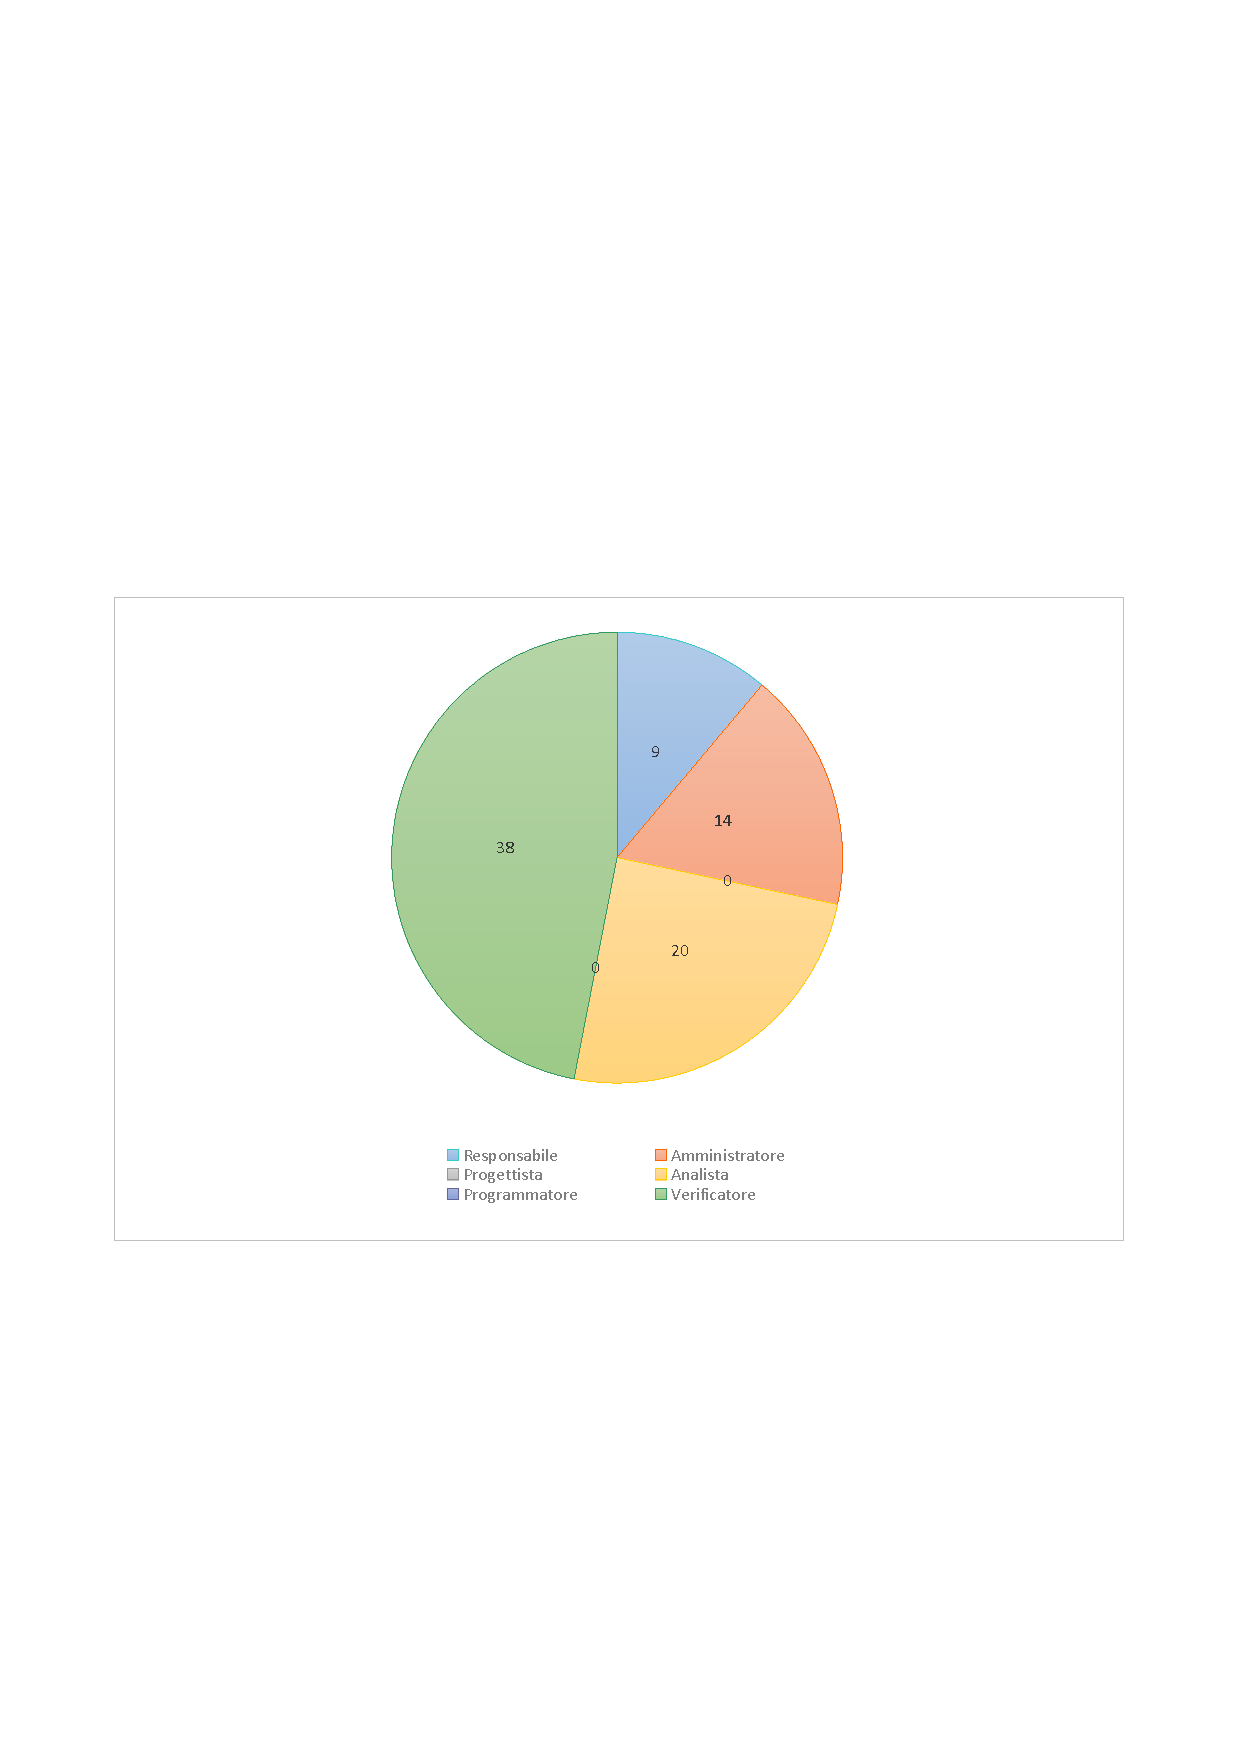
\includegraphics[width=0.93\textwidth , trim=2cm 9.5cm 2cm 11cm]{grafici/AD/AD-ore-ruolo}
			\caption{Fase AD - Ore per ruolo}
		\label{fig:CircleChart-faseAD_ore_r}
	\end{figure}
\vfill
	\begin{figure}[!h]
		\centering
		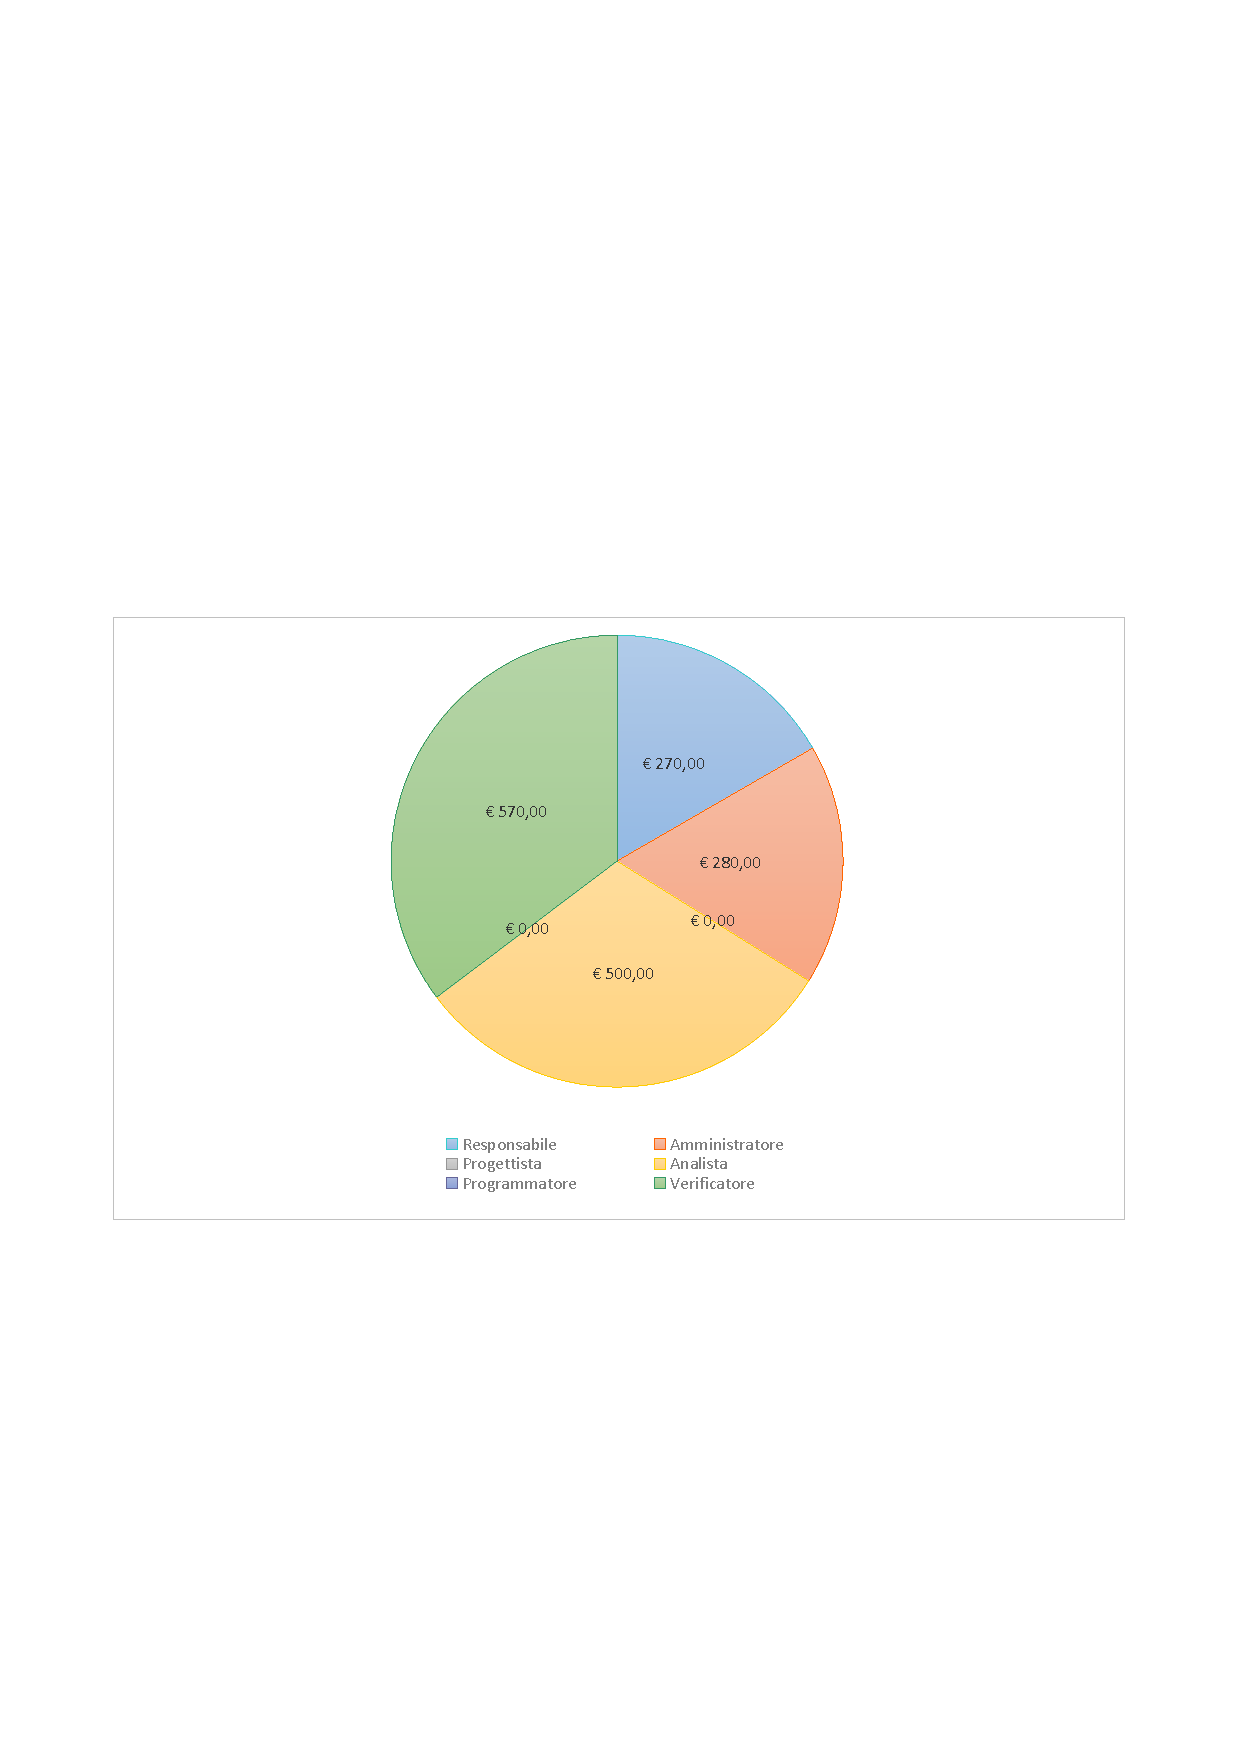
\includegraphics[width=0.93\textwidth , trim=2cm 9.5cm 2cm 11cm]{grafici/AD/AD-costo}
			\caption{Fase AD - Costo per ruolo}
		\label{fig:CircleChart-faseAD_costo}
	\end{figure}
\vfill		
\newpage	
	\subsubsection{Fase PA}
				\paragraph{Suddivisione del lavoro}
						
	\begin{table}[h]
		\centering
	
		\begin{tabularx}{\textwidth}{l  * {6}{C}  c}
			\toprule
			\textbf{Nominativo} & \textbf{Rp} & \textbf{Am} & \textbf{Pt} 
						& \textbf{An} & \textbf{Pm} & \textbf{Ve} & \textbf{Ore totali} \\
			\midrule
			Andrighetto Cristian & 0 & 0 &	17 & 10 & 0 & 0 & 27 \\
			%\midrule
			Bicego Eduard & 0 & 0 & 0 & 23 & 0 & 6 & 29 \\
			%\midrule
			Castello Davide & 0 & 0 & 0 & 24 & 0 & 2 & 26 \\
			%\midrule
			Conti Oscar Elia & 0 & 0 &	19 & 0 & 0 & 10 & 29 \\
			%\midrule
			Tavella Federico &	0 & 7 & 20 & 0 & 0 & 0 & 27 \\
			%\midrule
			Tombolato Andrea & 0 & 5 &	17 & 0 & 0 & 5 & 27 \\
			%\midrule
			Zanella Marco & 20 & 0 & 0 & 5 & 0 & 0 & 25 \\
			\midrule			
			Ore Totali Ruolo & 20 & 12 & 73 & 62 & 0 & 23 & 190 \\
			\bottomrule
			
		\end{tabularx}
		\caption{Fase PA - Suddivisione delle ore di lavoro}
		\label{tab:fasePA_ore}
	\end{table}
\vfill	
	
	\begin{figure}[!h]
		\centering
		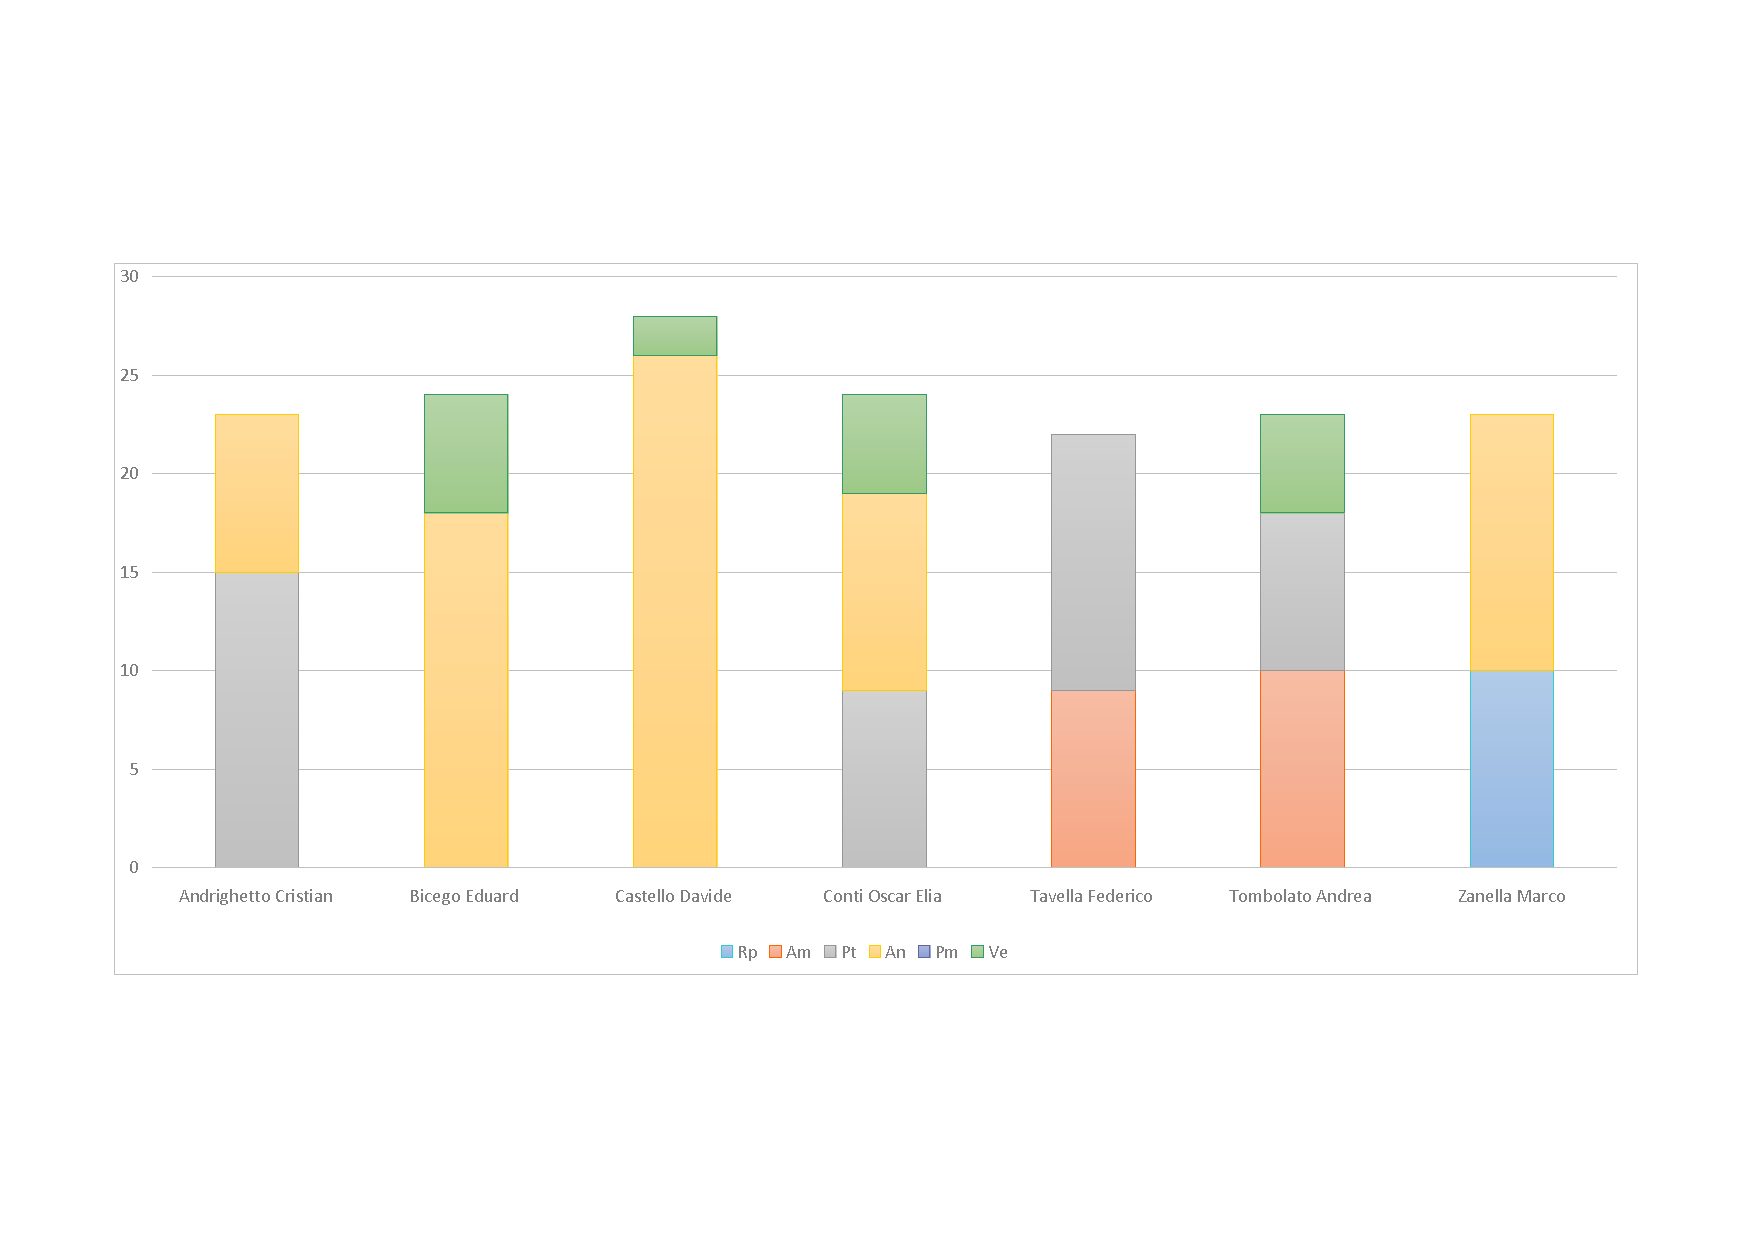
\includegraphics[width=\textwidth , trim=2cm 5cm 2cm 5cm]{grafici/PA/PA-ore-persona}
			\caption{Fase PA - Riassunto}
		\label{fig:BarChart-fasePA_ore}
	\end{figure}
\vfill	
\newpage
	
	\paragraph{Prospetto economico}
					
	\begin{table}[h]
		\centering
	
		\begin{tabular}{l * {2}{c}}
			\toprule
			\textbf{Ruolo} & \textbf{Ore} & \textbf{Costo (\euro{})} \\
			\midrule
			Responsabile &	20 & 600,00 \\
			%\midrule
			Amministratore & 12 & 240,00 \\
			%\midrule
			Progettista & 73 & 1.606,00 \\
			%\midrule
			Analista & 62 & 1.550,00 \\
			%\midrule
			Programmatore & 0 & 0,00 \\
			%\midrule
			Verificatore & 23 & 345,00 \\
			\midrule		
			\textbf{Totale} & 190 & 4.341,00 \\
			\bottomrule
		\end{tabular}
		\caption{Fase PA - Costo per ruolo}
		\label{tab:fasePA_costo}
	\end{table}
\vfill	
	
	\begin{figure}[!h]
		\centering
		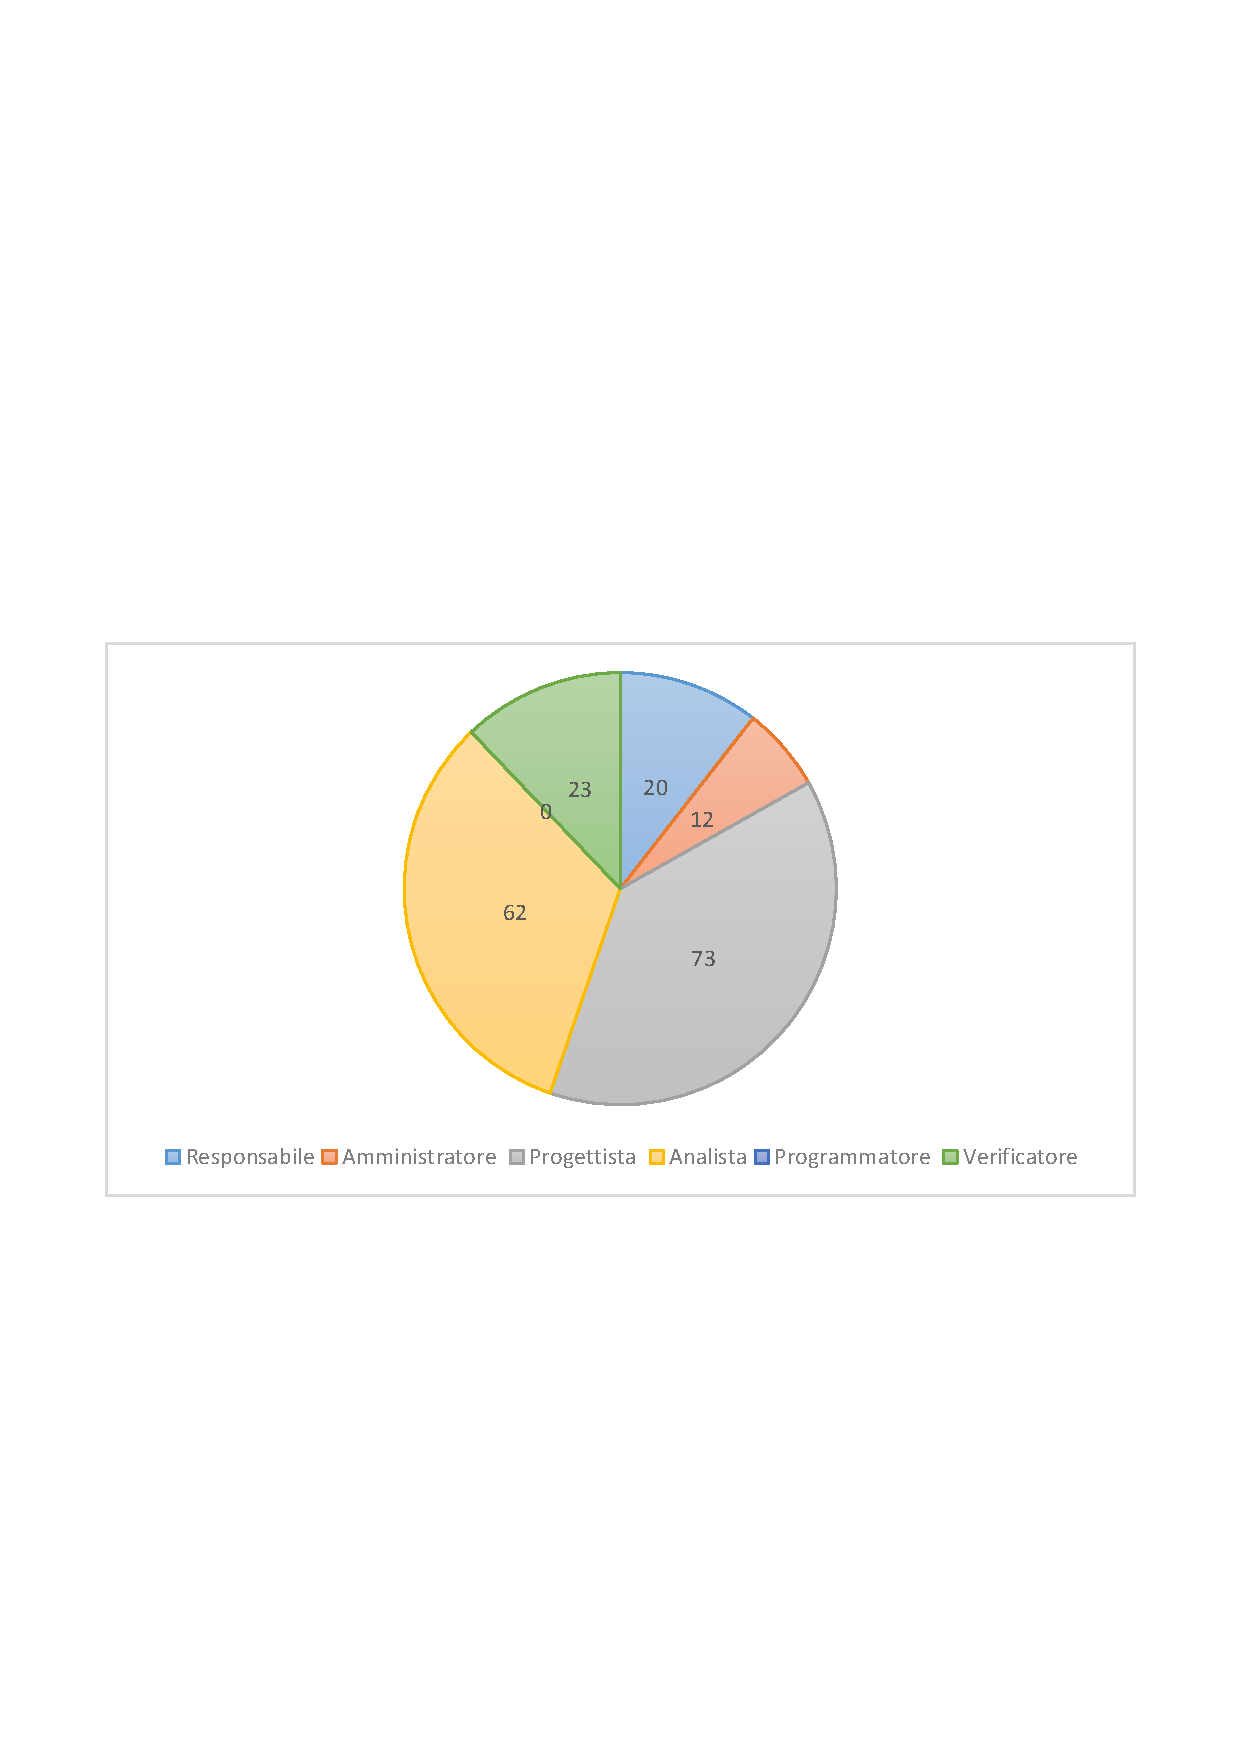
\includegraphics[width=0.93\textwidth , trim=2cm 9.5cm 2cm 11cm]{grafici/PA/PA-ore-ruolo}
			\caption{Fase PA - Ore per ruolo}
		\label{fig:CircleChart-fasePA_ore_r}
	\end{figure}
\vfill	
\newpage
\vfill
	\begin{figure}[!h]
		\centering
		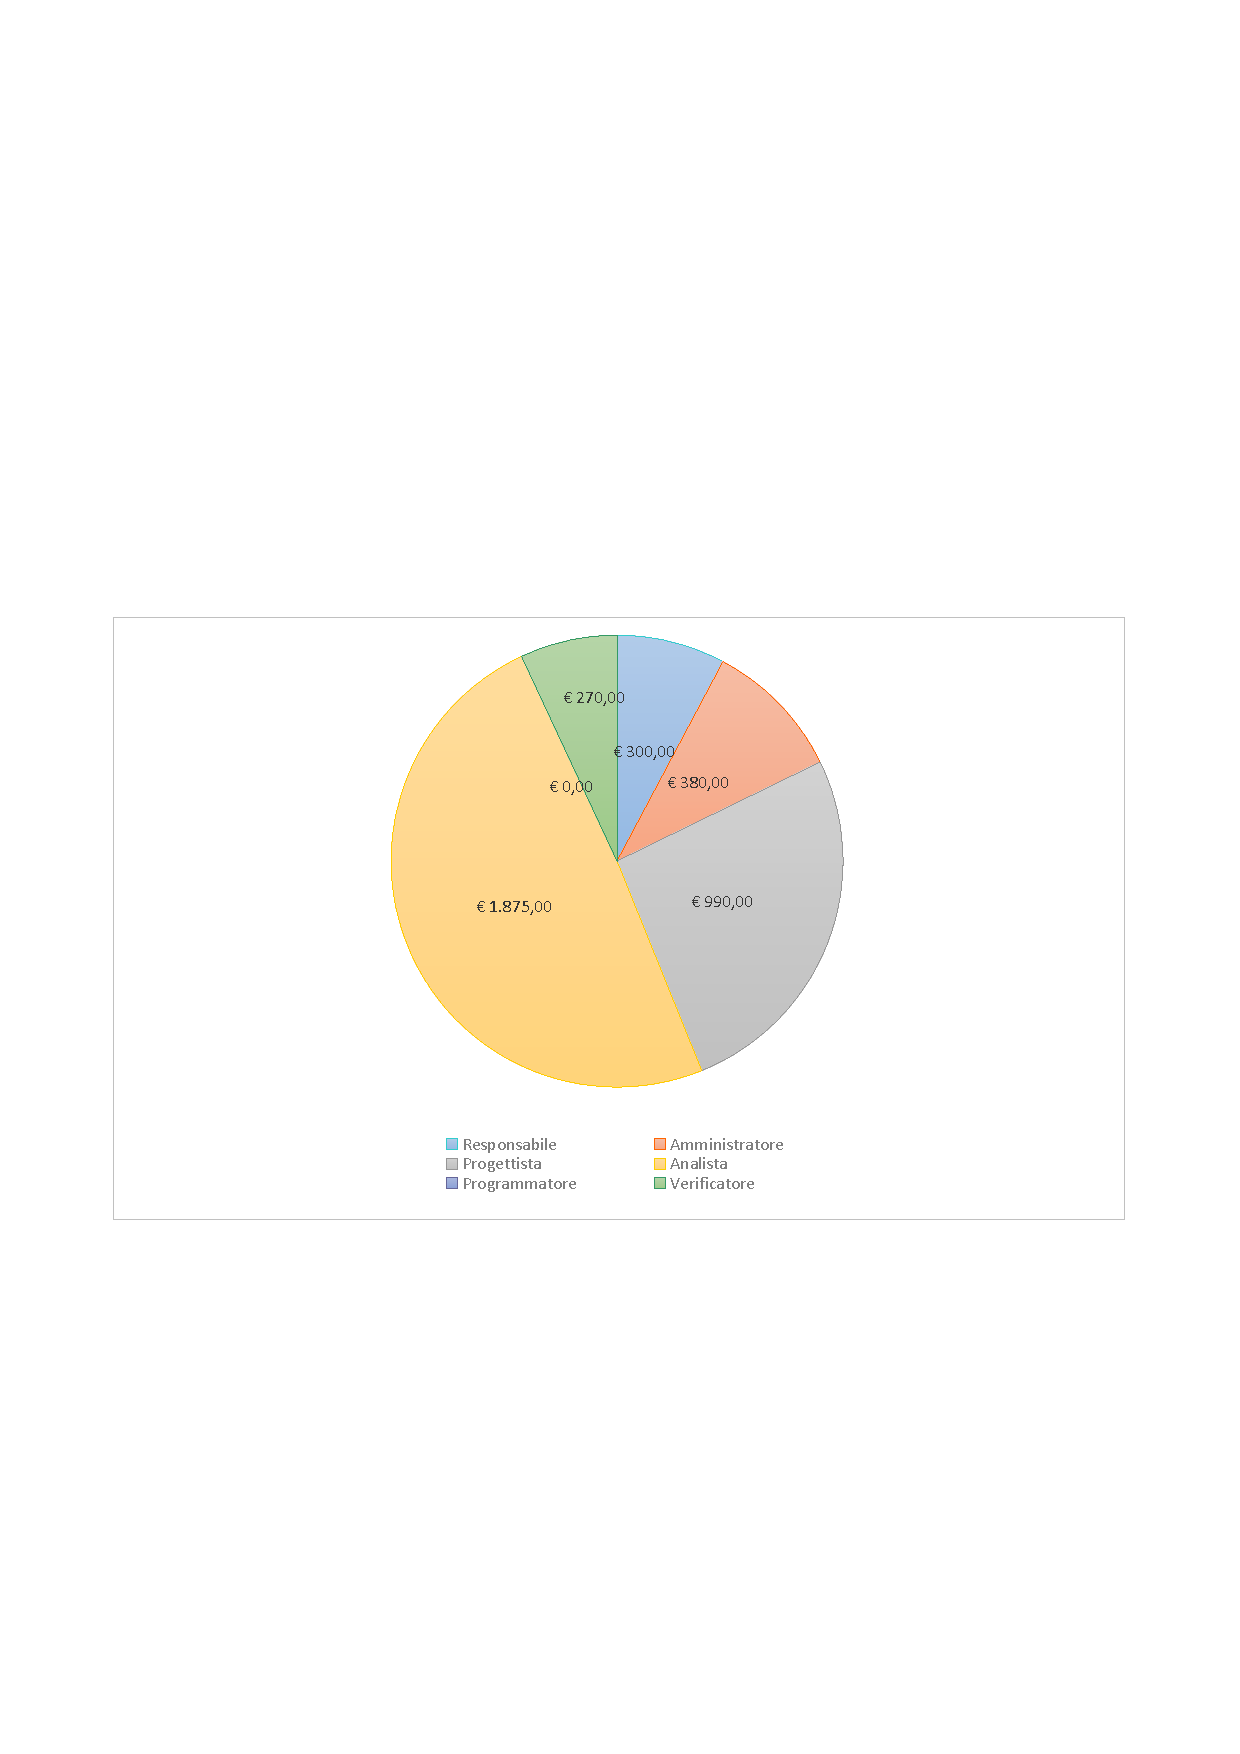
\includegraphics[width=0.93\textwidth , trim=2cm 9.5cm 2cm 11cm]{grafici/PA/PA-costo}
			\caption{Fase PA - Costo per ruolo}
		\label{fig:CircleChart-fasePA_costo}
	\end{figure}	
\vfill	
	\subsubsection{Fase PDROB}
				\paragraph{Suddivisione del lavoro}
					
	
	\begin{table}[h]
		%\centering
	
		\begin{tabularx}{\textwidth}{l  * {6}{C}  c}
			\toprule
			\textbf{Nominativo} & \textbf{Rp} & \textbf{Am} & \textbf{Pt} 
						& \textbf{An} & \textbf{Pm} & \textbf{Ve} & \textbf{Ore totali} \\
			\midrule
			Andrighetto Cristian & 0 &	0 &	0 &	19 & 0 & 15 & 34 \\
			%\midrule
			Bicego Eduard & 0 &	0 &	20 & 0 & 12 & 0 & 32 \\
			%\midrule
			Castello Davide & 0 & 10 & 23 &	0 &	0 &	0 &	33 \\
			%\midrule
			Conti Oscar Elia & 17 &	0 &	10 & 0 & 5 & 0 & 32 \\
			%\midrule
			Tavella Federico &	0 &	0 &	0 &	0 &	10 & 15 & 25 \\
			%\midrule
			Tombolato Andrea & 0 & 0 &	15 & 0 & 10 & 6 & 31 \\
			%\midrule
			Zanella Marco & 0 & 0 &	21 & 0 & 12 & 0 & 33 \\
			\midrule			
			\textbf{Ore Totali Ruolo} & 17 & 10 & 89 & 19 & 49 &	36 & 220 \\
			\bottomrule
		\end{tabularx}
		\caption{Fase PDROB - Suddivisione delle ore di lavoro}
		\label{tab:fasePDROB_ore}
	\end{table}
\vfill
\newpage
\vfill	
		
	\begin{figure}[!h]
		\centering
		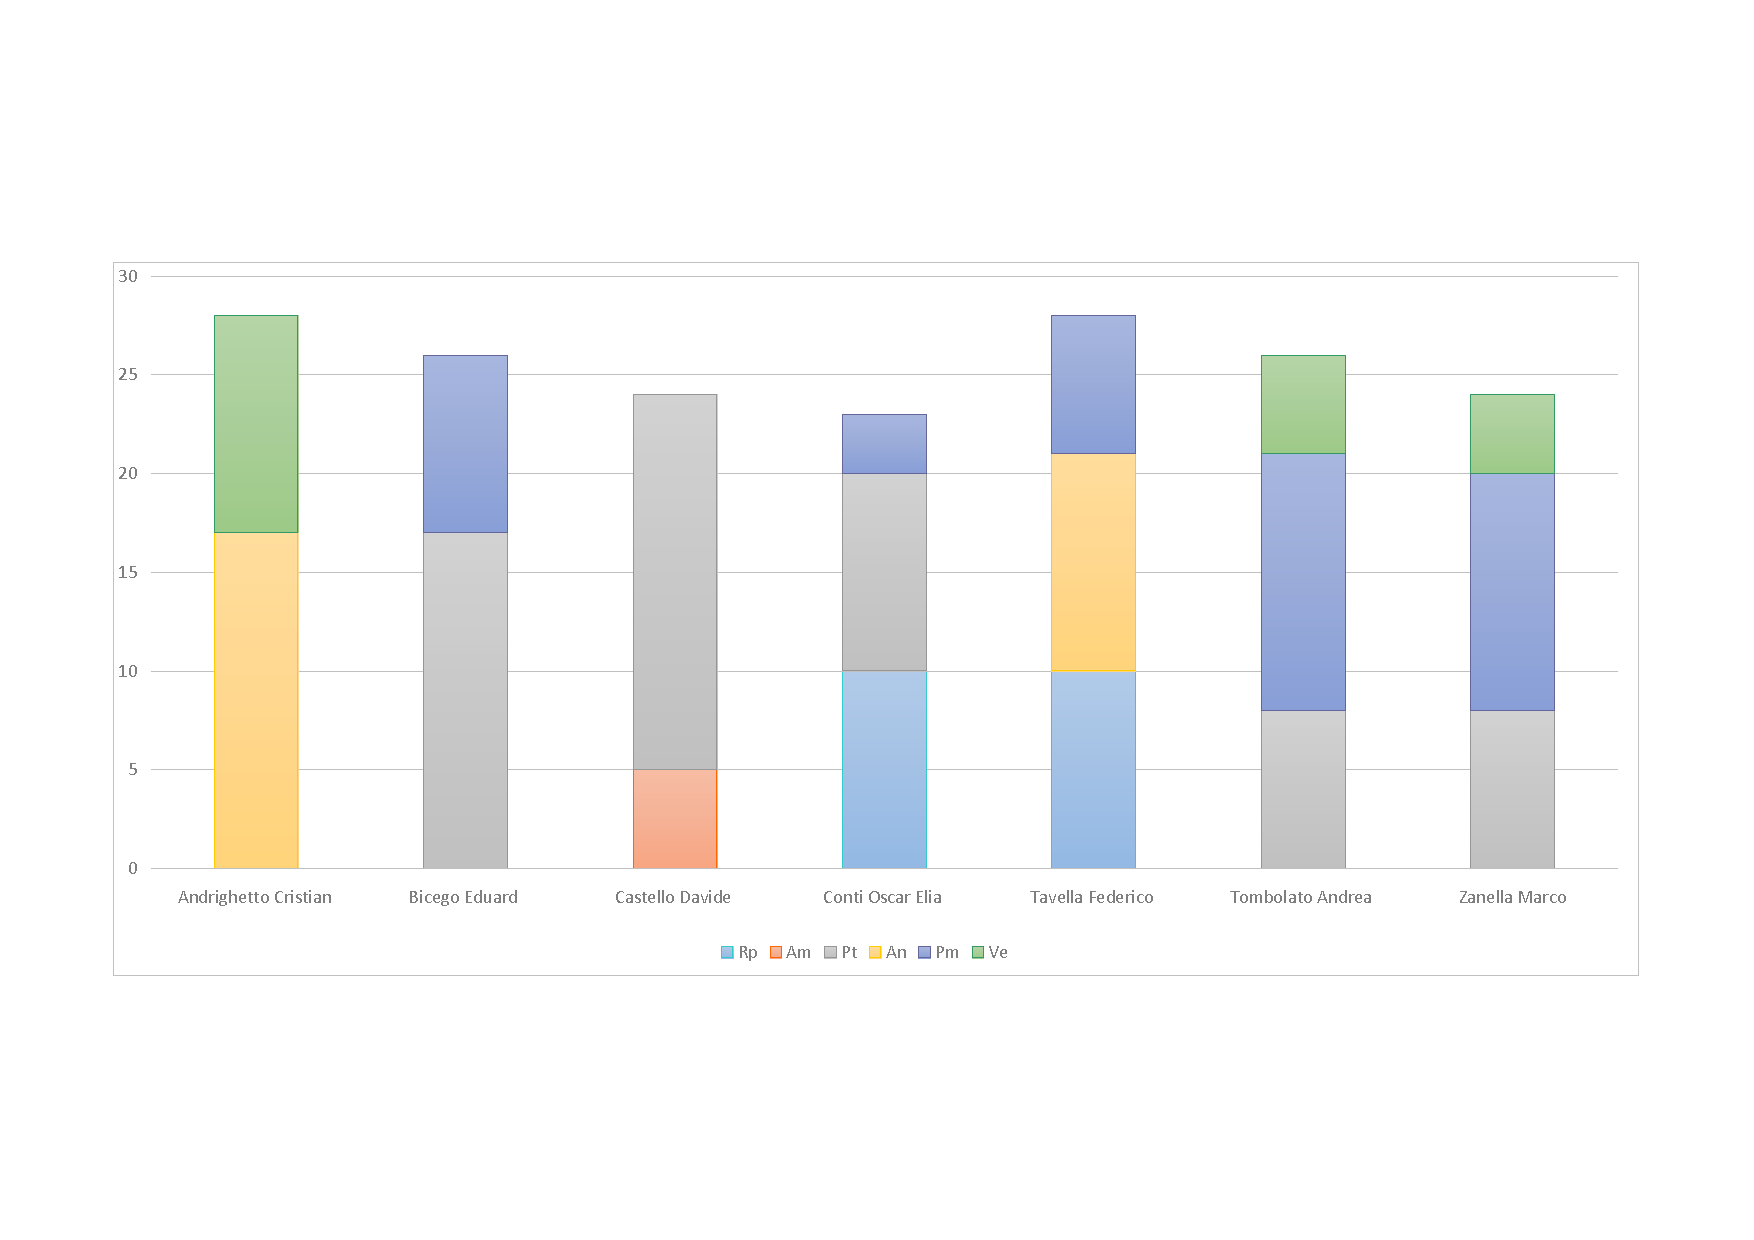
\includegraphics[width=\textwidth , trim=2cm 5cm 2cm 5cm]{grafici/PDROB/PDROB-ore-persona}
			\caption{Fase PDROB - Riassunto}
		\label{fig:BarChart-fasePDROB_ore}
	\end{figure}
\vfill	
	\paragraph{Prospetto economico}
					
	\begin{table}[h]
		\centering
	
		\begin{tabular}{l * {2}{c}}
			\toprule
			\textbf{Ruolo} & \textbf{Ore} & \textbf{Costo (\euro{})} \\
			\midrule
			Responsabile &	17 & 510,00 \\
			%\midrule
			Amministratore & 10 & 200,00 \\
			%\midrule
			Progettista & 89 & 1.958,00 \\
			%\midrule
			Analista & 19 & 475,00 \\
			%\midrule
			Programmatore & 49 & 735,00 \\
			%\midrule
			Verificatore & 36 & 540,00 \\
			\midrule		
			\textbf{Totale} & 220 & 4.418,00 \\
			\bottomrule	
		\end{tabular}
		\caption{Fase PDROB - Costo per ruolo}
		\label{tab:fasePDROB_costo}
	\end{table}
\vfill	
\newpage
\vfill
	
	\begin{figure}[!h]
		\centering
		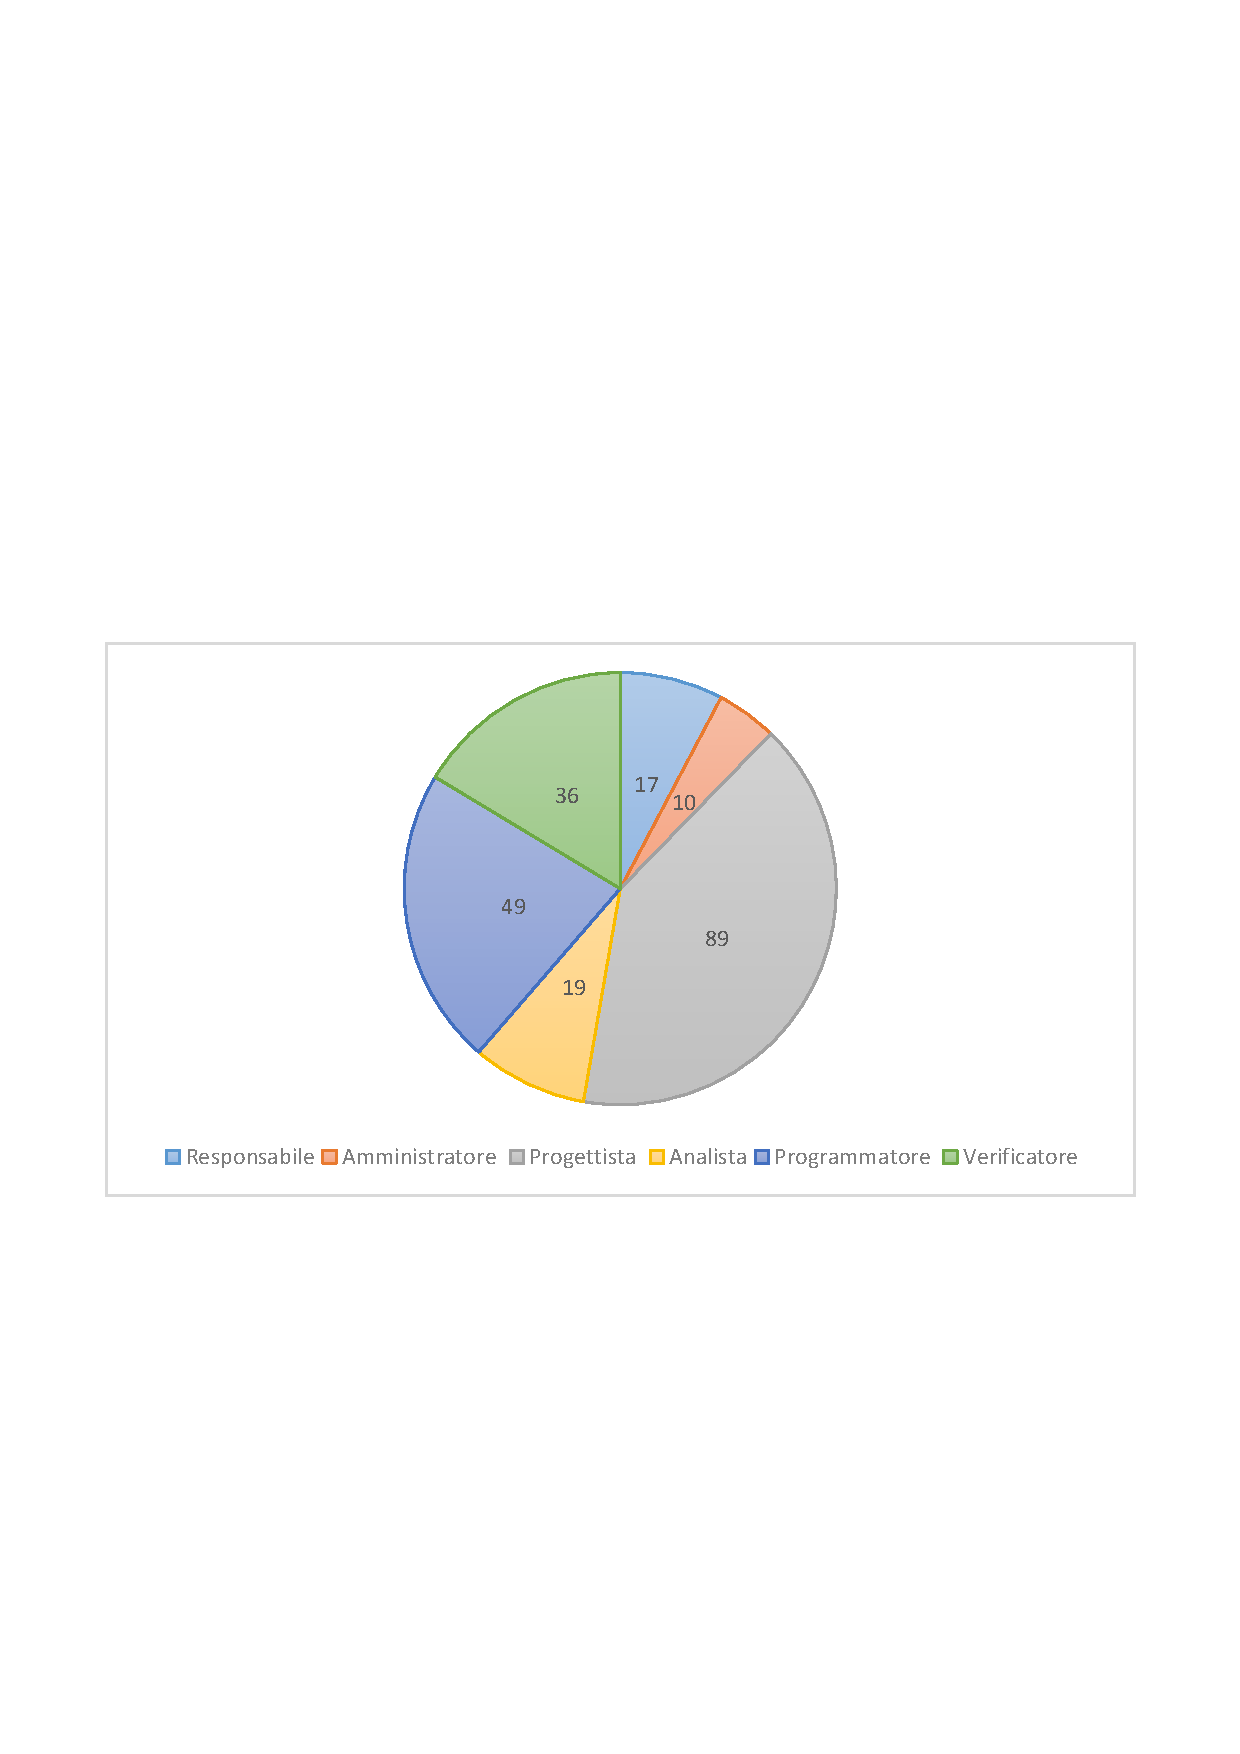
\includegraphics[width=0.93\textwidth , trim=2cm 9.5cm 2cm 11cm]{grafici/PDROB/PDROB-ore-ruolo}
			\caption{Fase PDROB - Ore per ruolo}
		\label{fig:CircleChart-fasePDROB_ore_r}
	\end{figure}

\vfill	
	\begin{figure}[!h]
		\centering
		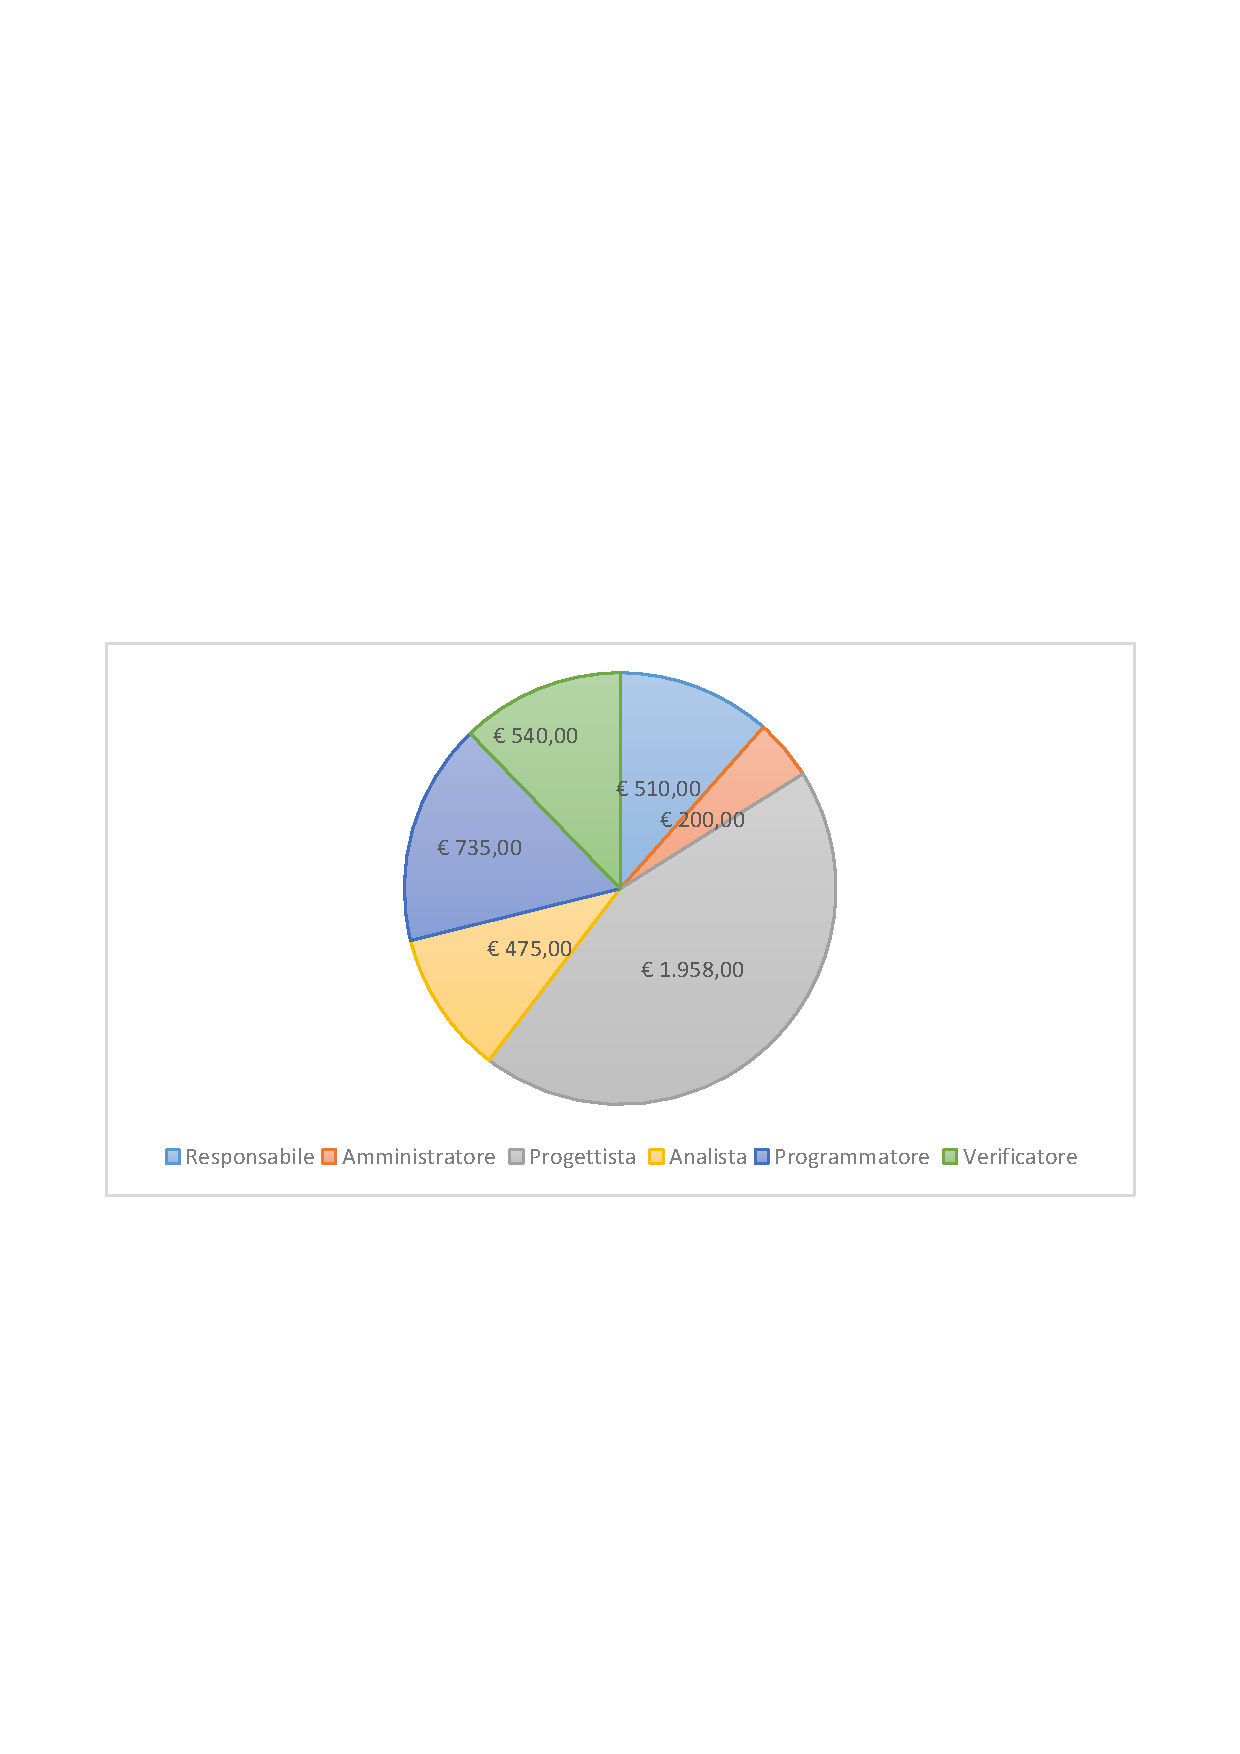
\includegraphics[width=0.93\textwidth , trim=2cm 9.5cm 2cm 11cm]{grafici/PDROB/PDROB-costo}
			\caption{Fase PDROB - Costo per ruolo}
		\label{fig:CircleChart-fasePDROB_costo}
	\end{figure}
\vfill	
\newpage	
	
	\subsubsection{Fase PDRD}
				\paragraph{Suddivisione del lavoro}
						
	\begin{table}[h]
		%\centering
	
		\begin{tabularx}{\textwidth}{l  * {6}{C}  c}
			\toprule
			\textbf{Nominativo} & \textbf{Rp} & \textbf{Am} & \textbf{Pt} 
						& \textbf{An} & \textbf{Pm} & \textbf{Ve} & \textbf{Ore totali} \\
			\midrule
			Andrighetto Cristian & 0 & 0 & 0 & 4 & 3 & 9 & 16 \\
			%\midrule
			Bicego Eduard & 0 & 5 &	0 &	7 &	0 &	3 &	15 \\
			%\midrule
			Castello Davide & 10 & 0 & 0 & 0 & 0 & 6 & 16 \\
			%\midrule
			Conti Oscar Elia & 0 & 0 & 0 & 0 & 10 &	4 &	14 \\
			%\midrule
			Tavella Federico &	0 & 0 &	0 &	0 &	8 &	7 &	15 \\
			%\midrule
			Tombolato Andrea & 0 & 0 & 5 & 0 & 0 & 9 & 14 \\
			%\midrule
			Zanella Marco & 0 & 0 & 5 &	2 &	0 &	8 &	15 \\
			\midrule			
			\textbf{Ore Totali Ruolo} & 10 & 5 & 10 & 13 &	21 & 46 & 105 \\
			\bottomrule
		\end{tabularx}
		\caption{Fase PDRD - Suddivisione delle ore di lavoro}
		\label{tab:fasePDRD_ore}
	\end{table}
\vfill	
		
	\begin{figure}[!h]
		\centering
		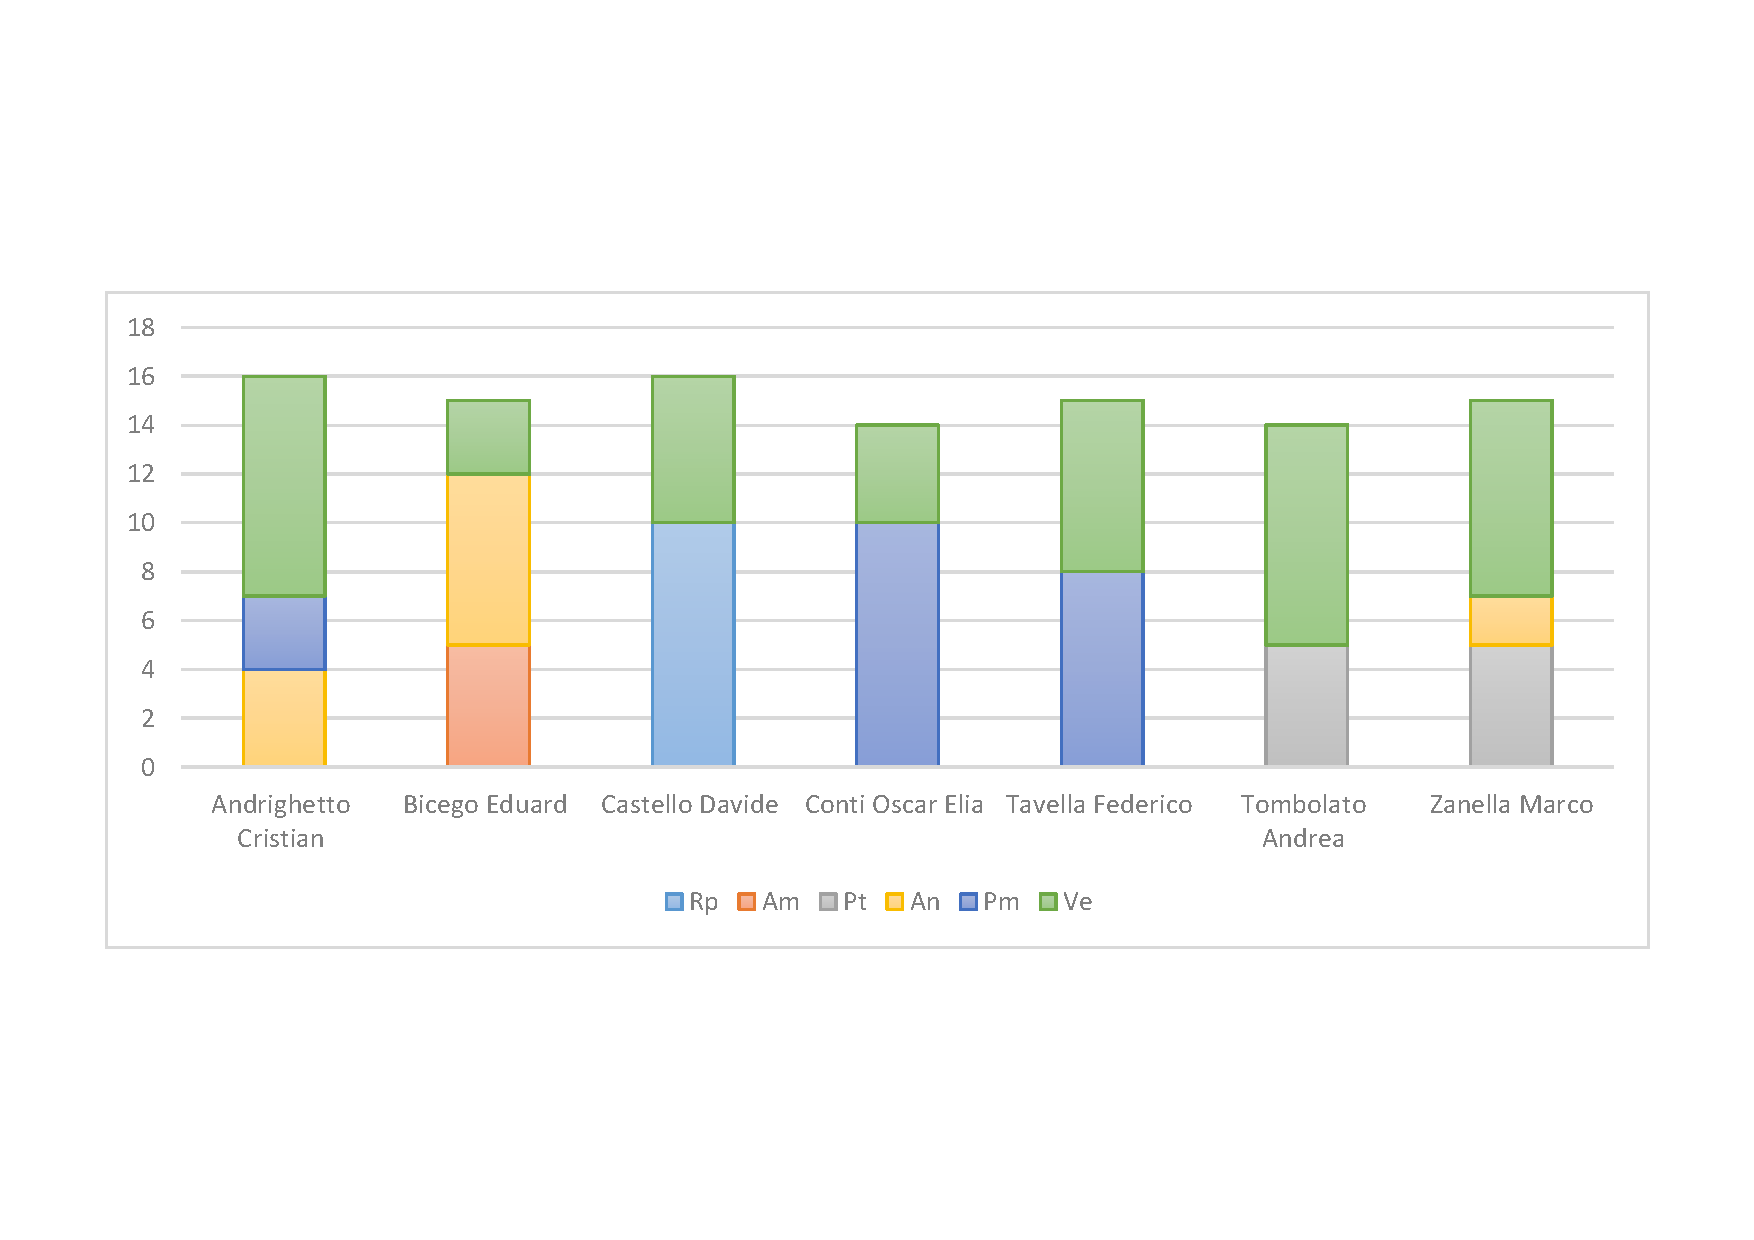
\includegraphics[width=\textwidth , trim=2cm 5cm 2cm 5cm]{grafici/PDRD/PDRD-ore-persona}
			\caption{Fase PDRD - Riassunto}
		\label{fig:BarChart-fasePDRD_ore}
	\end{figure}
\vfill	
\newpage	
	
	\paragraph{Prospetto economico}
					
	\begin{table}[h]
		\centering
	
		\begin{tabular}{l * {2}{c}}
			\toprule
			\textbf{Ruolo} & \textbf{Ore} & \textbf{Costo (\euro{})} \\
			\midrule
			Responsabile &	10 & 300,00 \\
			%\midrule
			Amministratore & 5 & 100,00 \\
			%\midrule
			Progettista & 10 & 220,00 \\
			%\midrule
			Analista & 13 & 325,00 \\
			%\midrule
			Programmatore & 21 & 315,00 \\
			%\midrule
			Verificatore & 46 & 690,00 \\
			\midrule		
			Totale & 105 & 1.950,00 \\
			\bottomrule
		\end{tabular}
		\caption{Fase PDRD - Costo per ruolo}
		\label{tab:fasePDRD_costo}
	\end{table}
\vfill	
	
	\begin{figure}[!h]
		\centering
		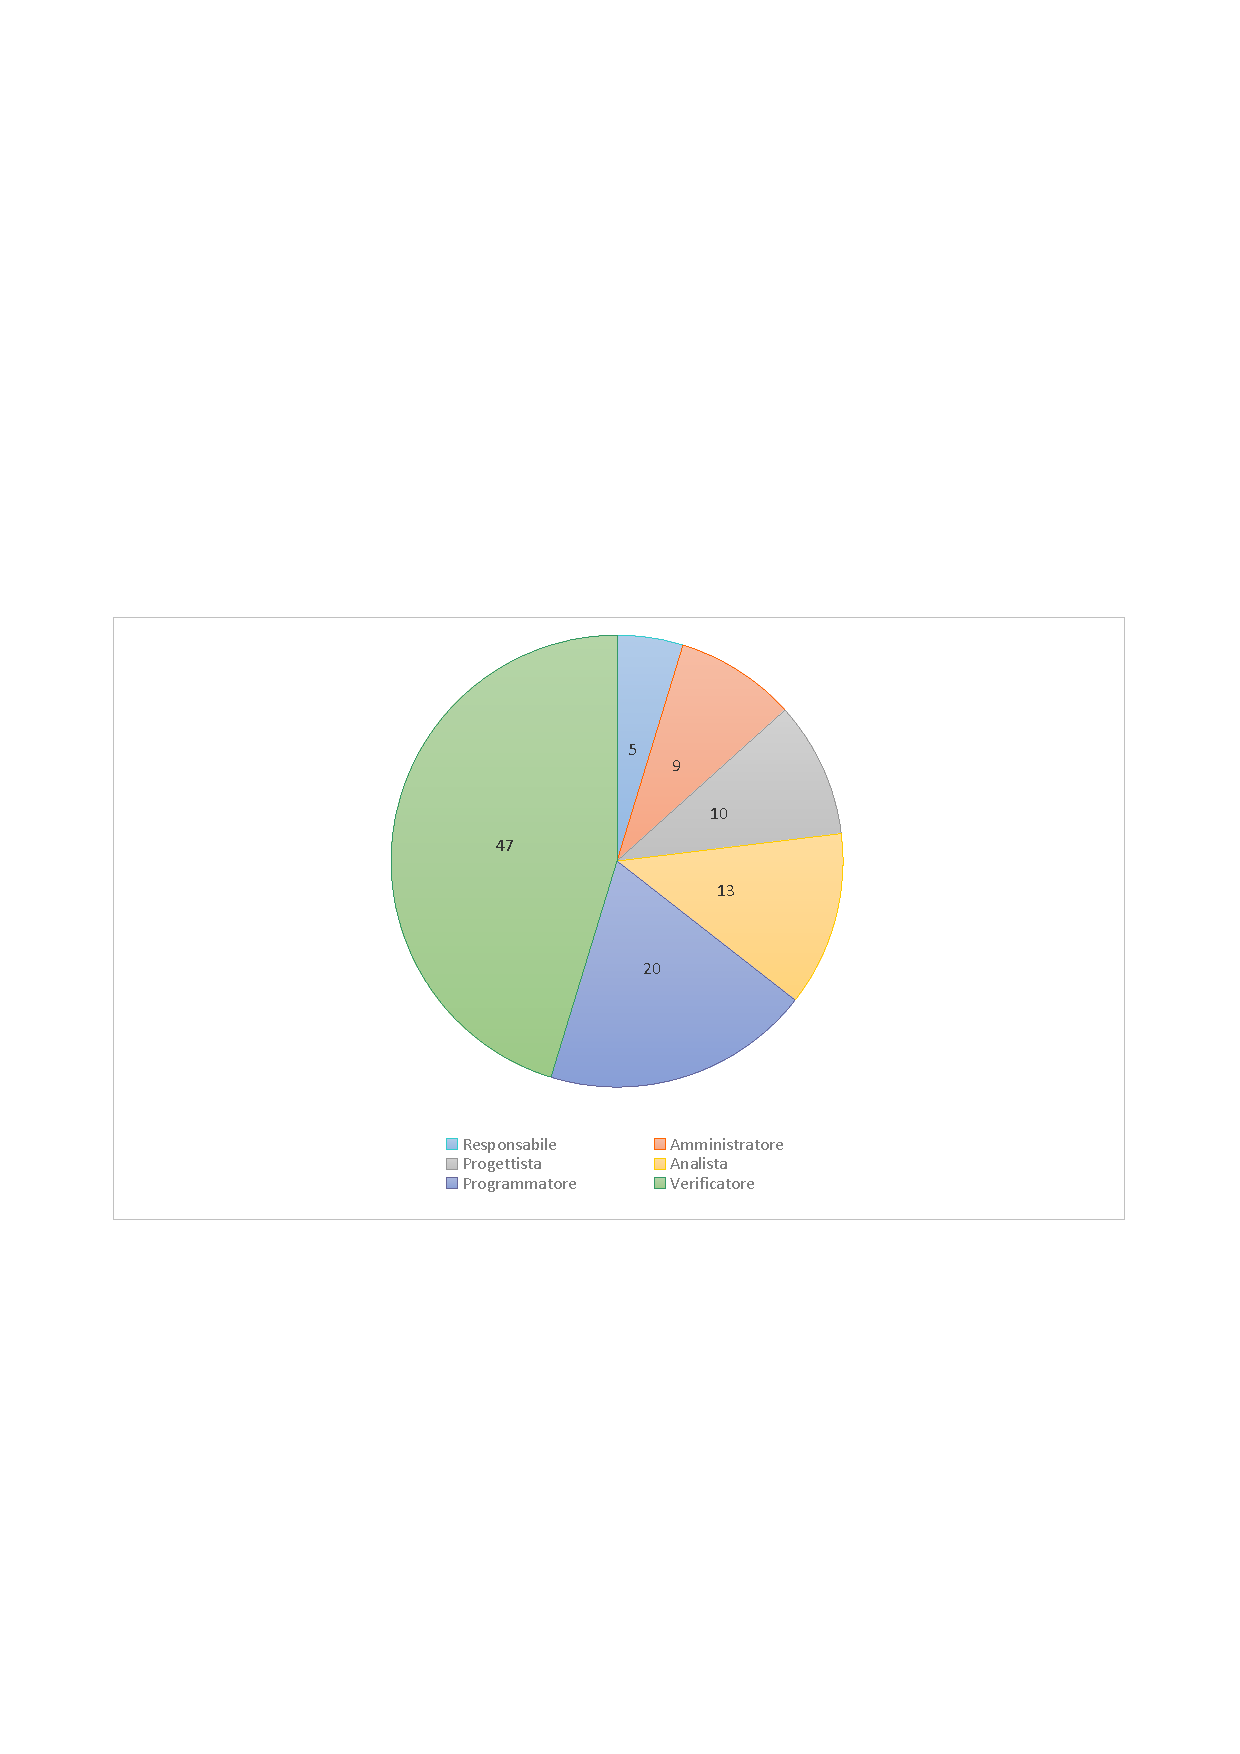
\includegraphics[width=0.93\textwidth , trim=2cm 9.5cm 2cm 11cm]{grafici/PDRD/PDRD-ore-ruolo}
			\caption{Fase PDRD - Ore per ruolo}
		\label{fig:CircleChart-fasePDRD_ore_r}
	\end{figure}
\vfill	
\newpage
\vfill
	\begin{figure}[!h]
		\centering
		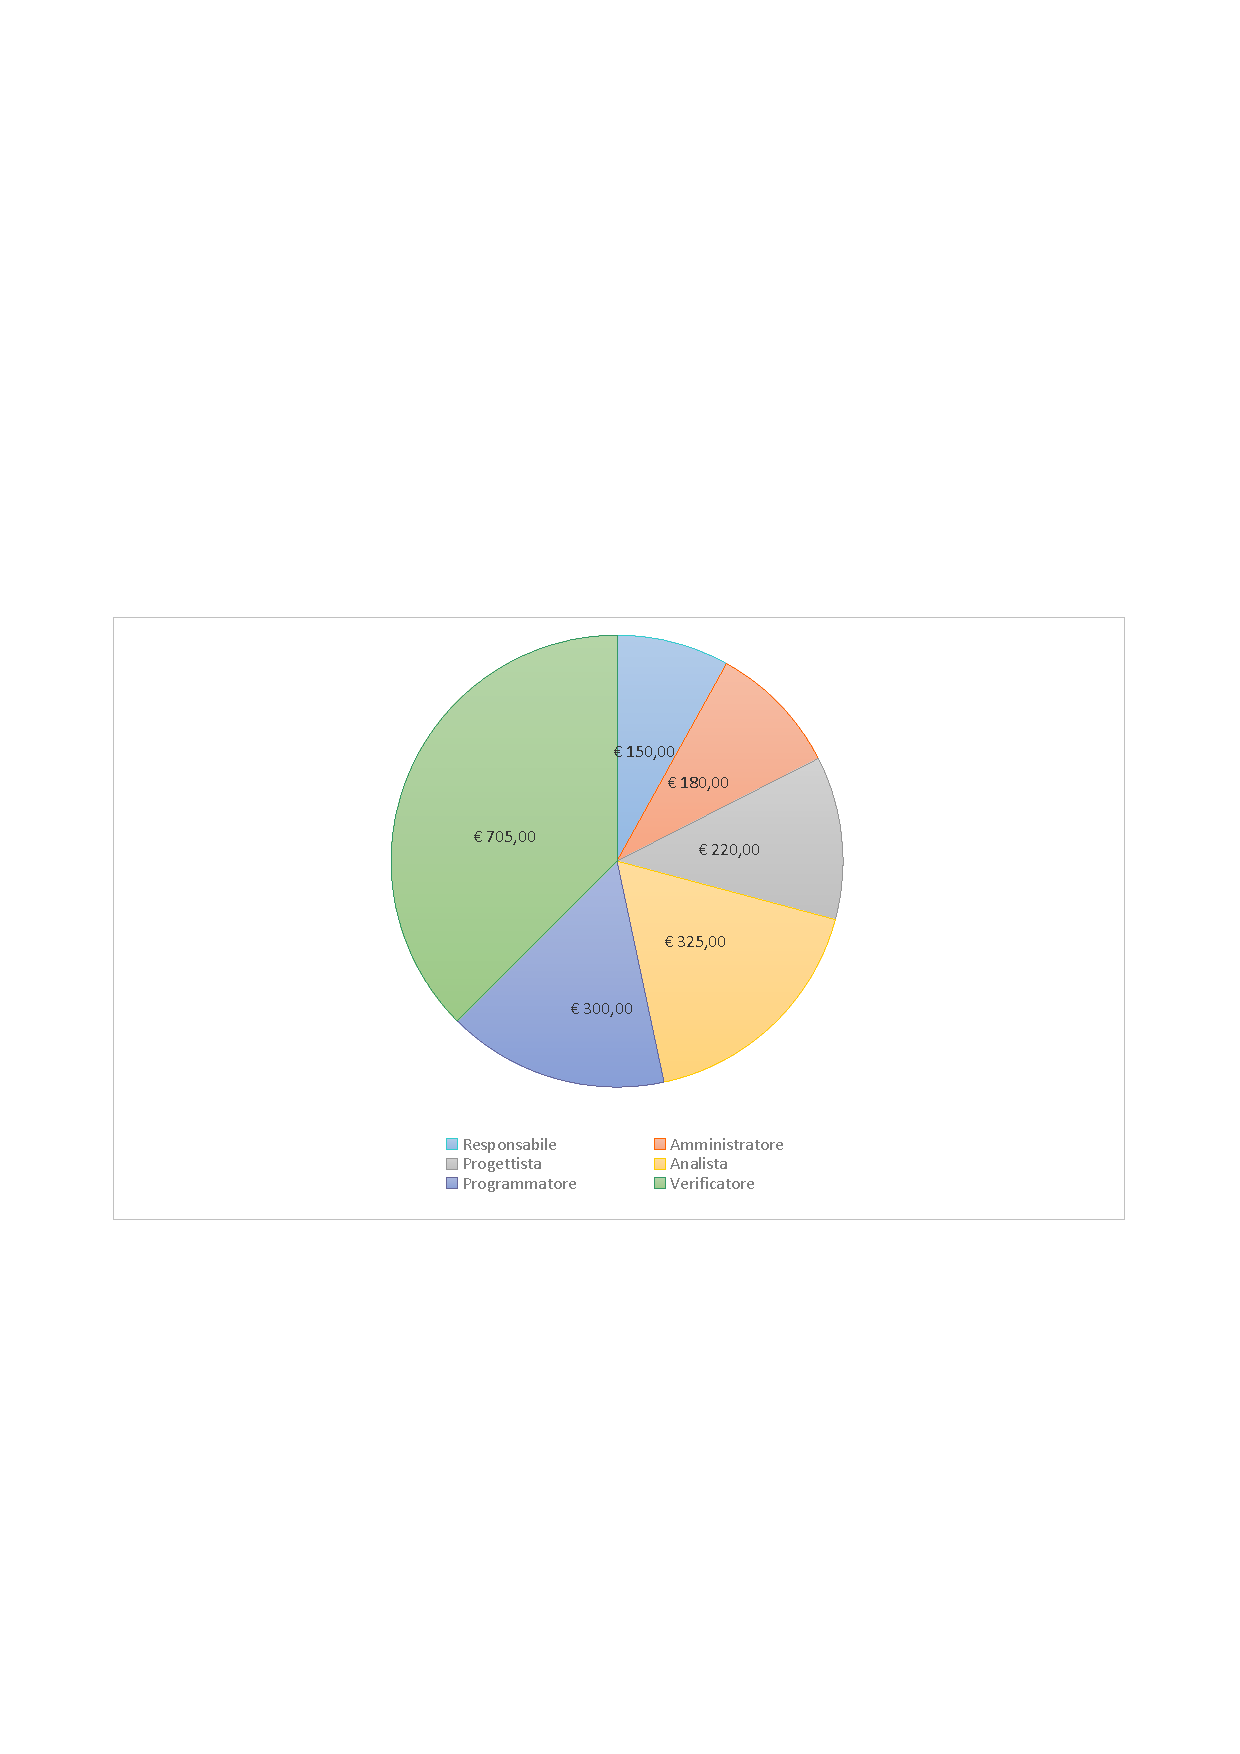
\includegraphics[width=0.93\textwidth , trim=2cm 9.5cm 2cm 11cm]{grafici/PDRD/PDRD-costo}
			\caption{Fase PDRD - Costo per ruolo}
		\label{fig:CircleChart-fasePDRD_costo_r}
	\end{figure}
\vfill
	
	\subsubsection{Fase PDROP}
				\paragraph{Suddivisione del lavoro}
						
	\begin{table}[h]
		%\centering
		\begin{tabularx}{\textwidth}{l  * {6}{C}  c}
			\toprule
			\textbf{Nominativo} & \textbf{Rp} & \textbf{Am} & \textbf{Pt} 
						& \textbf{An} & \textbf{Pm} & \textbf{Ve} & \textbf{Ore totali} \\
			\midrule
			Andrighetto Cristian & 0 & 0 & 0 & 0 & 6 & 7 & 13 \\
			%\midrule
			Bicego Eduard & 5 & 0 &	3 &	0 &	4 &	0 &	12 \\
			%\midrule
			Castello Davide & 0 & 0 & 7 & 0 & 0 & 5 & 12 \\
			%\midrule
			Conti Oscar Elia &0 & 4 & 7 & 3 & 0 & 0 & 14 \\
			%\midrule
			Tavella Federico &	0 & 0 & 6 & 0 & 0 & 6 & 12 \\
			%\midrule
			Tombolato Andrea & 0 & 0 & 6 & 2 & 7 & 0 & 15 \\
			%\midrule
			Zanella Marco & 0 & 7 & 0 & 5 & 0 & 0 & 12 \\
			\midrule			
			\textbf{Ore Totali Ruolo} & 5 & 11 & 29 & 10 & 17 & 18 & 90 \\
			\bottomrule
		\end{tabularx}
		\caption{Fase PDROP - Suddivisione delle ore di lavoro}
		\label{tab:fasePDROP_ore}
	\end{table}
	
\newpage
\vfill	
		
	\begin{figure}[!h]
		\centering
		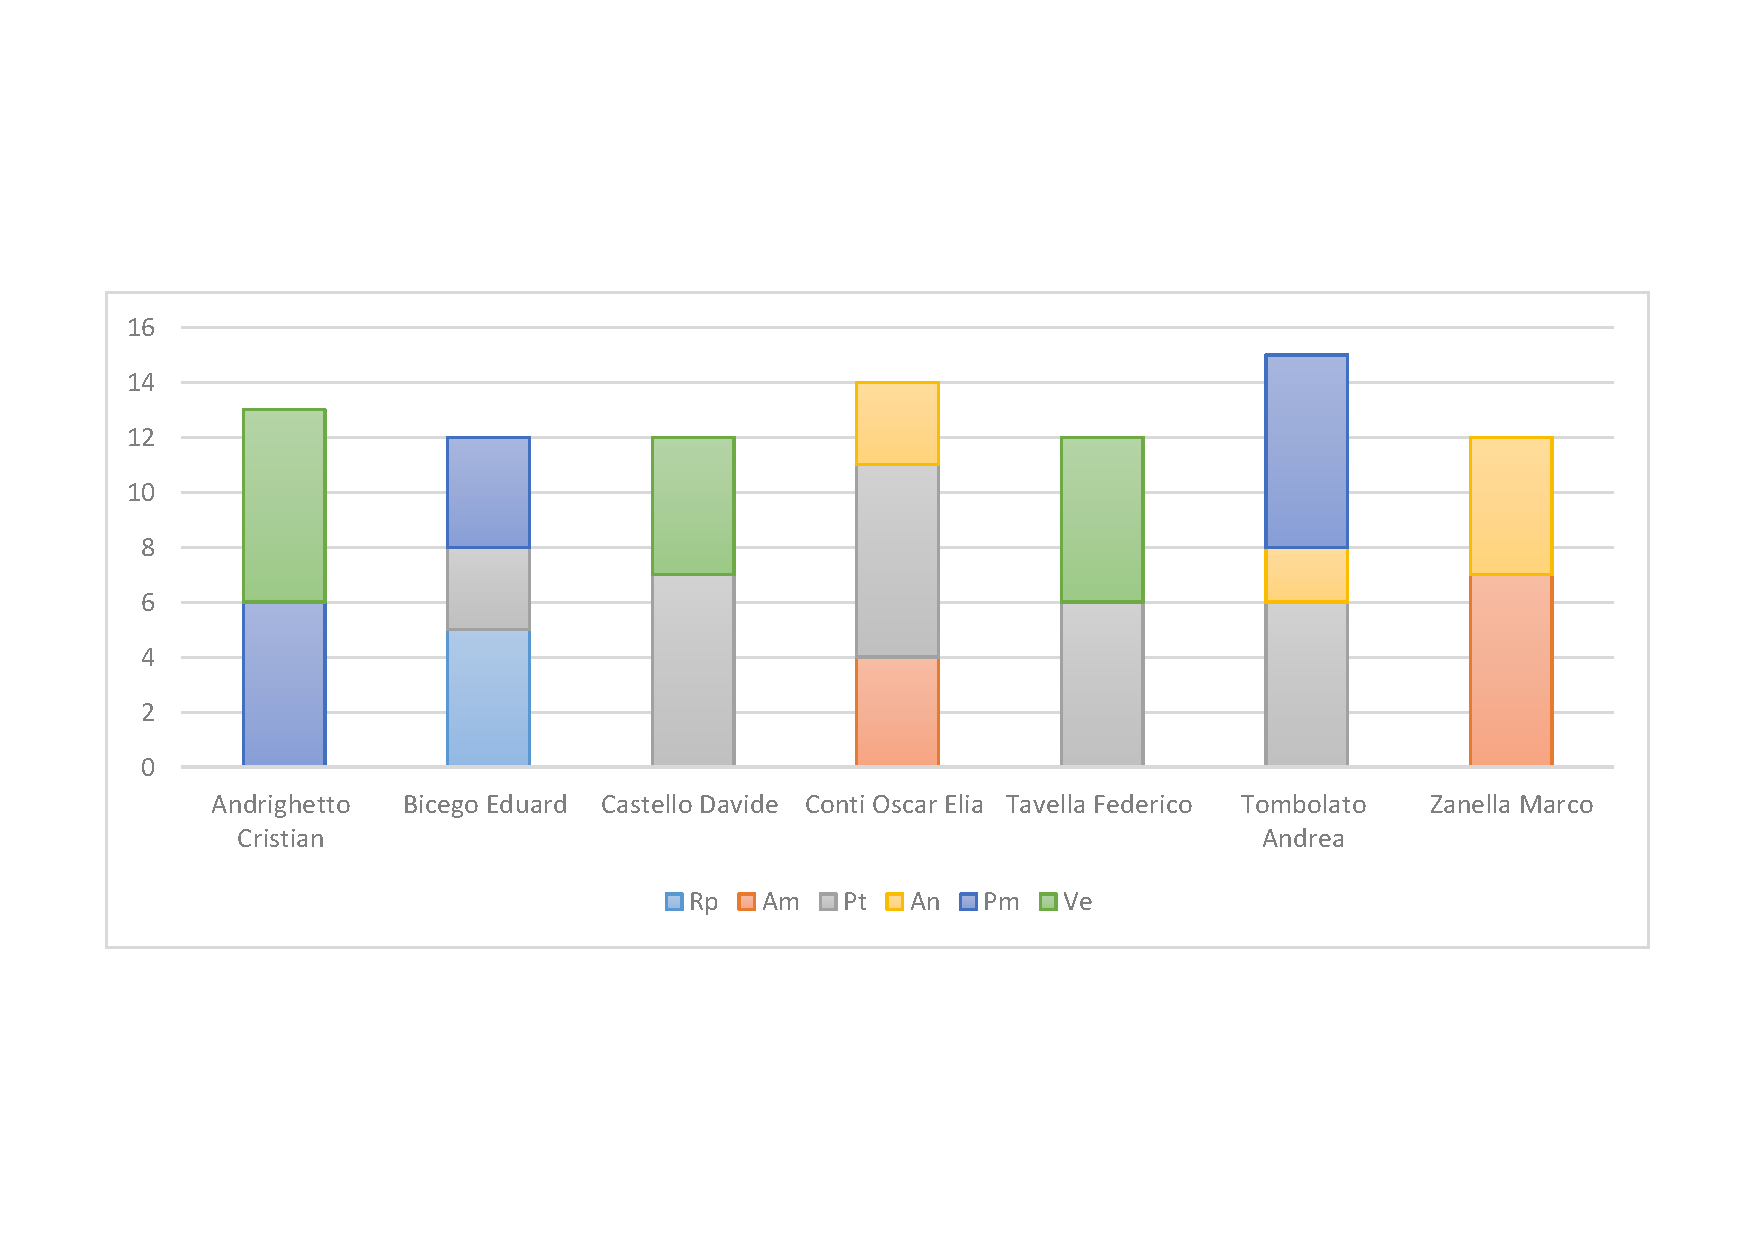
\includegraphics[width=\textwidth , trim=2cm 5cm 2cm 5cm]{grafici/PDROP/PDROP-ore-persona}
			\caption{Fase PDROP - Riassunto}
		\label{fig:BarChart-fasePDROP_ore}
	\end{figure}
\vfill	
	
	\paragraph{Prospetto economico}
					
	\begin{table}[h]
		\centering
	
		\begin{tabular}{l * {2}{c}}
			\toprule
			\textbf{Ruolo} & \textbf{Ore} & \textbf{Costo (\euro{})} \\
			\midrule
			Responsabile &	5 & 150,00 \\
			%\midrule
			Amministratore & 11 & 220,00 \\
			%\midrule
			Progettista & 29 & 638,00 \\
			%\midrule
			Analista & 10 & 250,00 \\
			%\midrule
			Programmatore & 17 & 255,00 \\
			%\midrule
			Verificatore & 18 & 270,00 \\
			\midrule		
			\textbf{Totale} & 90 & 1.783,00 \\
			\bottomrule
		\end{tabular}
		\caption{Fase PDROP - Costo per ruolo}
		\label{tab:fasePDROP_costo}
	\end{table}
\vfill	
\newpage
\vfill	
	
	\begin{figure}[!h]
		\centering
		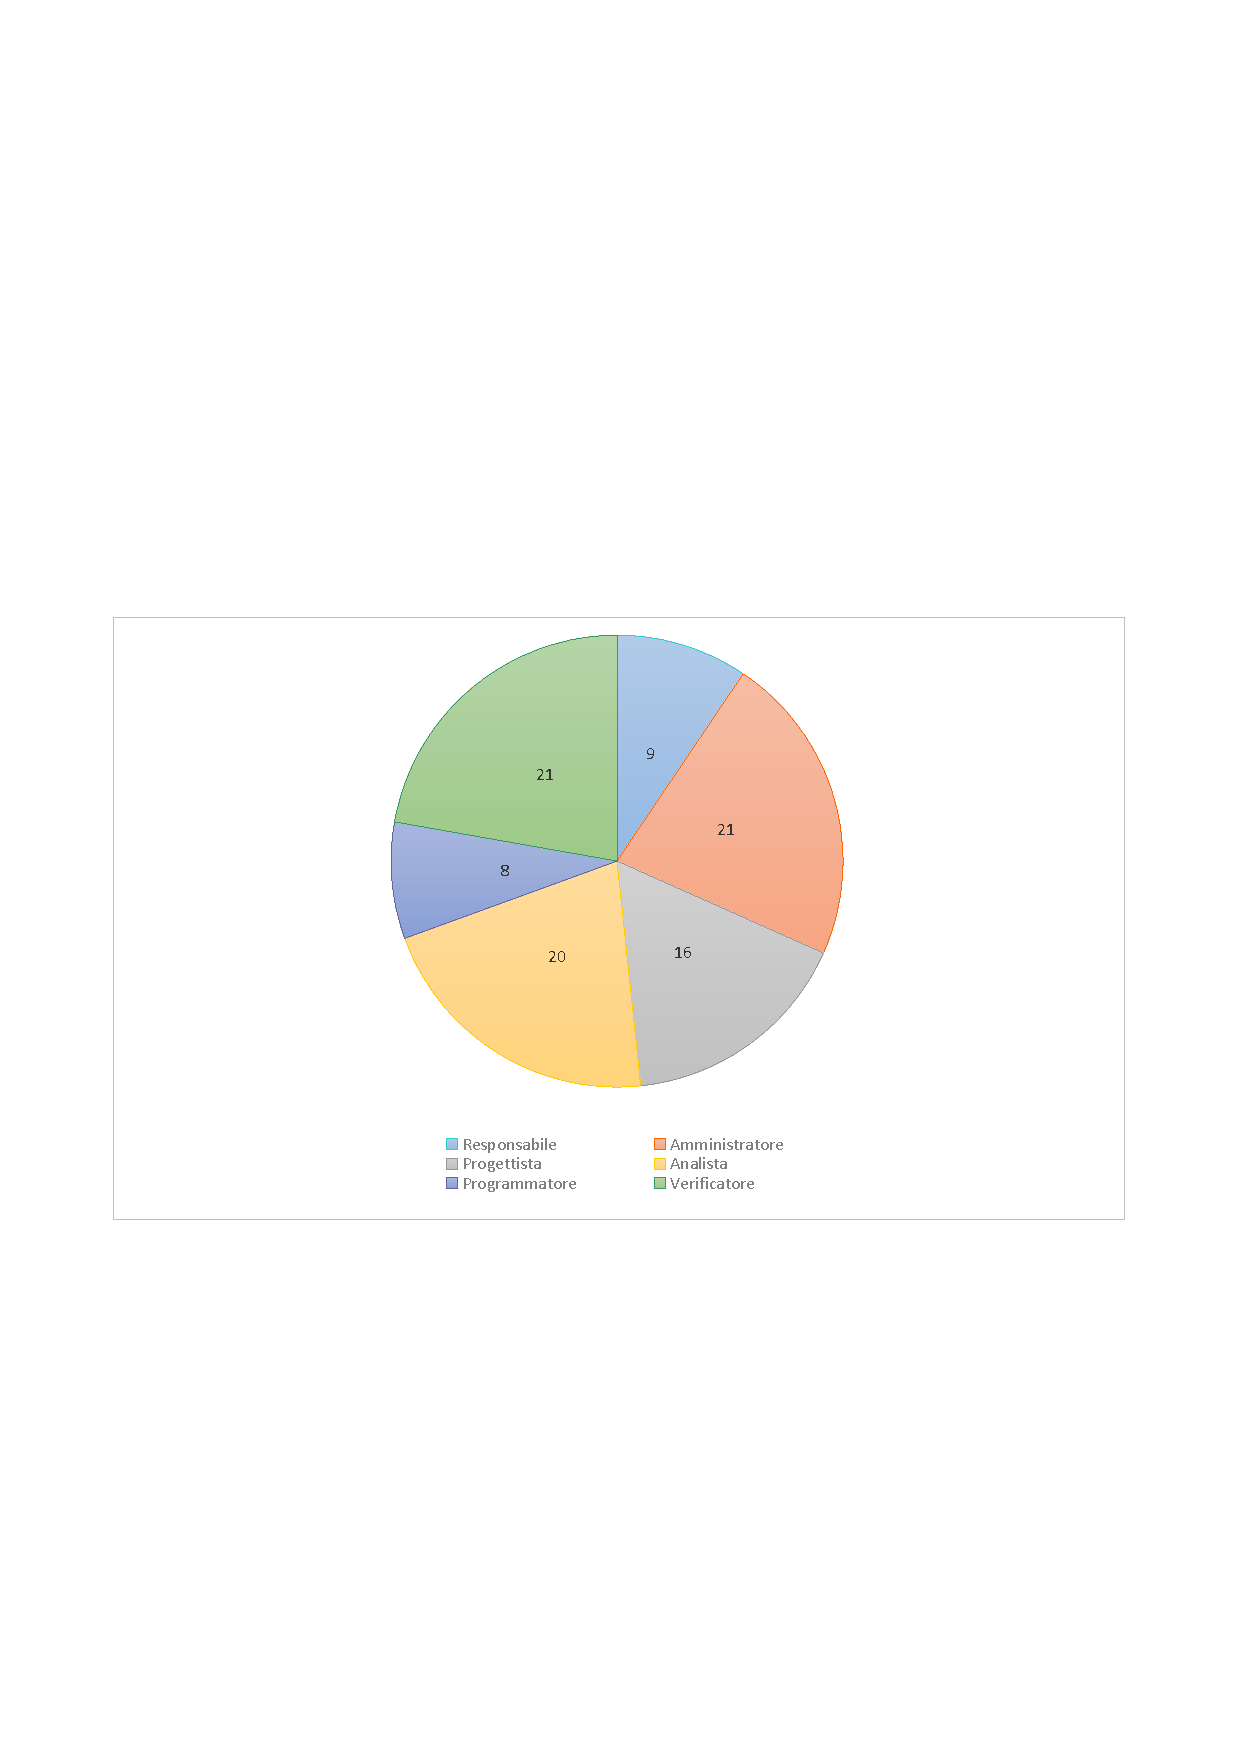
\includegraphics[width=0.93\textwidth , trim=2cm 9.5cm 2cm 11cm]{grafici/PDROP/PDROP-ore-ruolo}
			\caption{Fase PDROP - Ore per ruolo}
		\label{fig:CircleChart-fasePDRD_ore_r}
	\end{figure}
\vfill
	\begin{figure}[!h]
		\centering
		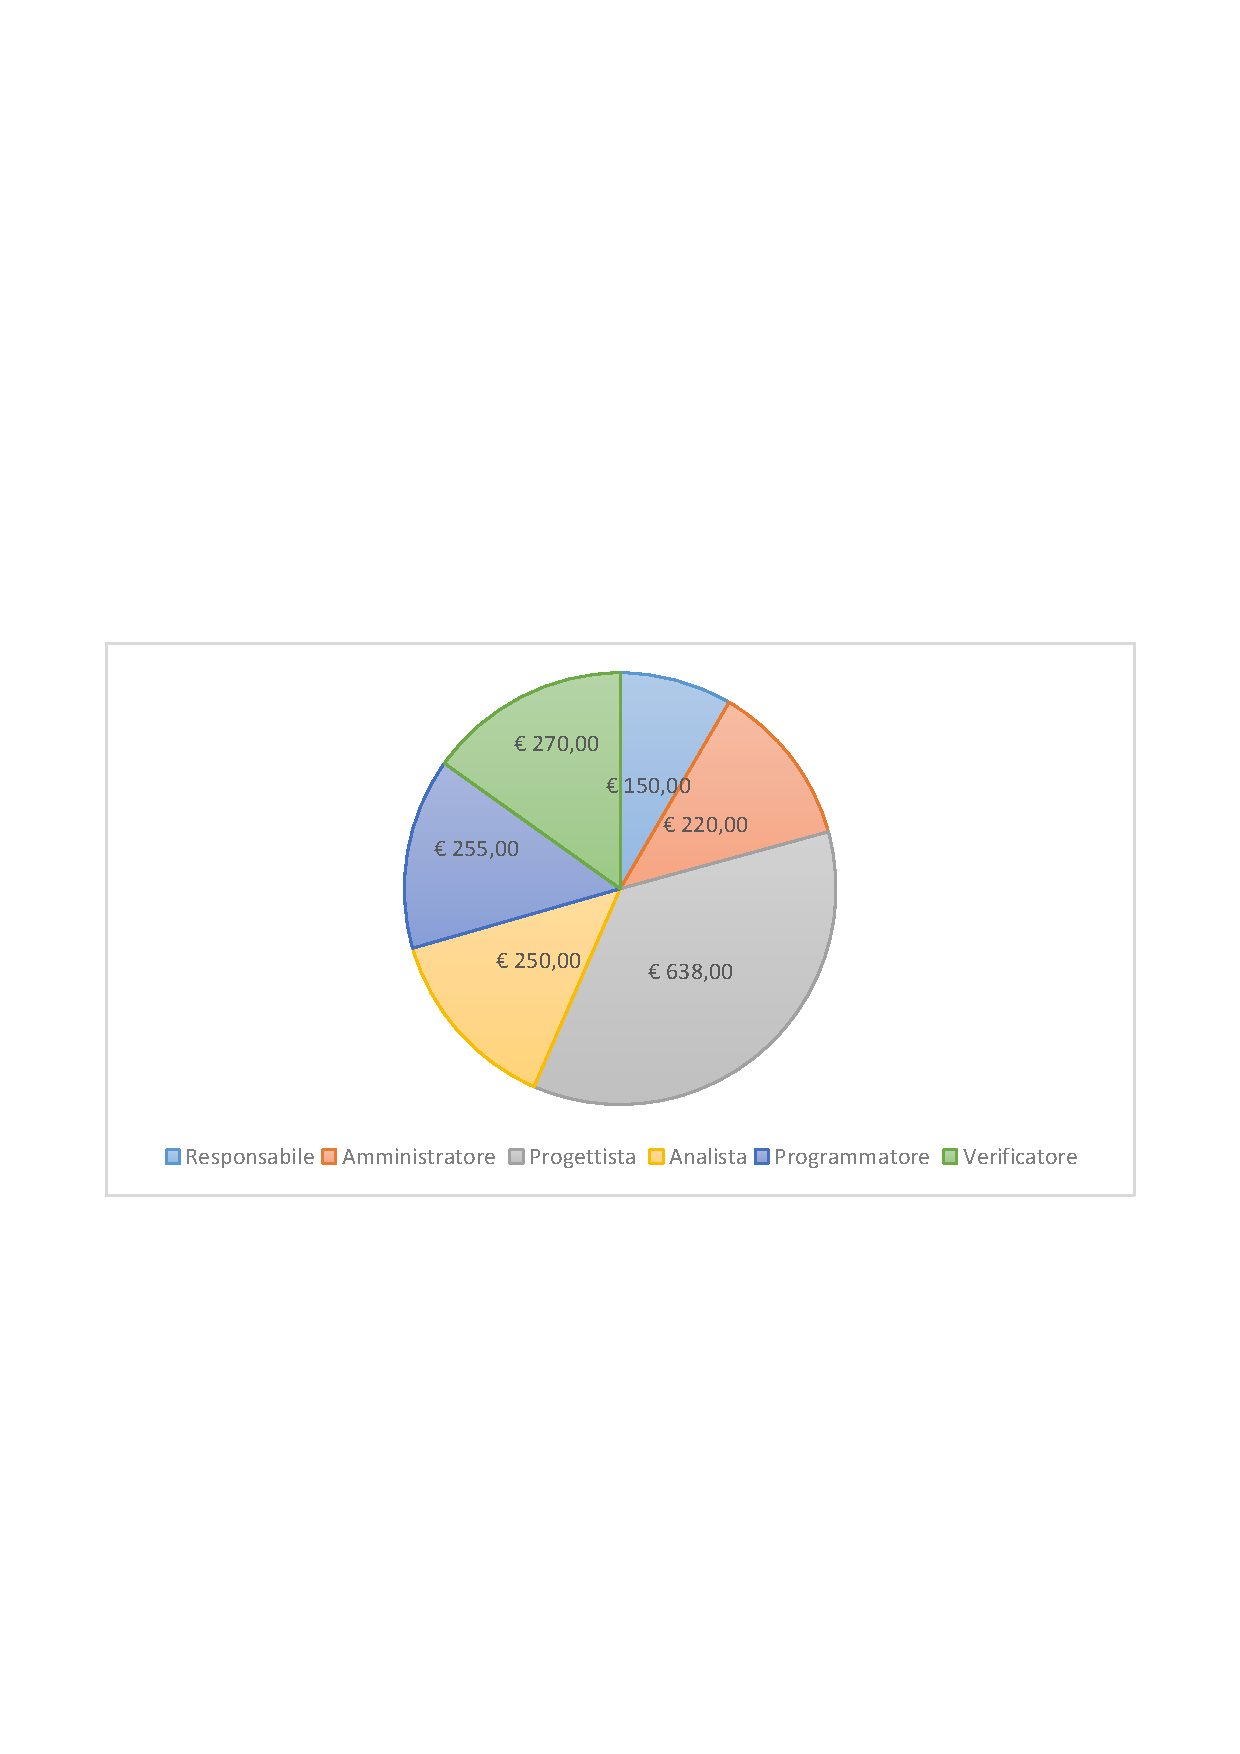
\includegraphics[width=0.93\textwidth , trim=2cm 9.5cm 2cm 11cm]{grafici/PDROP/PDROP-costo}
			\caption{Fase PDROP - Costo per ruolo}
		\label{fig:CircleChart-fasePDROP_costo}
	\end{figure}
\vfill	
\newpage
	
	\subsubsection{Fase V}
				\paragraph{Suddivisione del lavoro}
					
	\begin{table}[h]
		%\centering
		\begin{tabularx}{\textwidth}{l  * {6}{C}  c}
			\toprule
			\textbf{Nominativo} & \textbf{Rp} & \textbf{Am} & \textbf{Pt} 
						& \textbf{An} & \textbf{Pm} & \textbf{Ve} & \textbf{Ore totali} \\
			\midrule
			Andrighetto Cristian & 0 & 4 & 0 & 0 & 0 & 10 & 14 \\
			%\midrule
			Bicego Eduard & 0 & 0 &	0 &	0 &	11 & 5 & 16 \\
			%\midrule
			Castello Davide & 0 & 0 & 0 & 0 & 9 & 7 & 16 \\
			%\midrule
			Conti Oscar Elia &0 & 0 & 0 & 0 & 0 & 9 & 9 \\
			%\midrule
			Tavella Federico &	0 & 0 & 0 & 0 & 0 & 11 & 11 \\
			%\midrule
			Tombolato Andrea & 10 & 0 & 0 & 0 & 4 & 5 & 19 \\
			%\midrule
			Zanella Marco & 0 & 0 & 7 & 0 & 0 & 8 & 15 \\
			\midrule			
			\textbf{Ore Totali Ruolo} & 10 & 4 &	7 &	0 &	24 & 55 & 100 \\
			\bottomrule
		\end{tabularx}
		\caption{Fase V - Suddivisione delle ore di lavoro}
		\label{tab:faseV_ore}
	\end{table}
\vfill	

	
	\begin{figure}[!h]
		\centering
		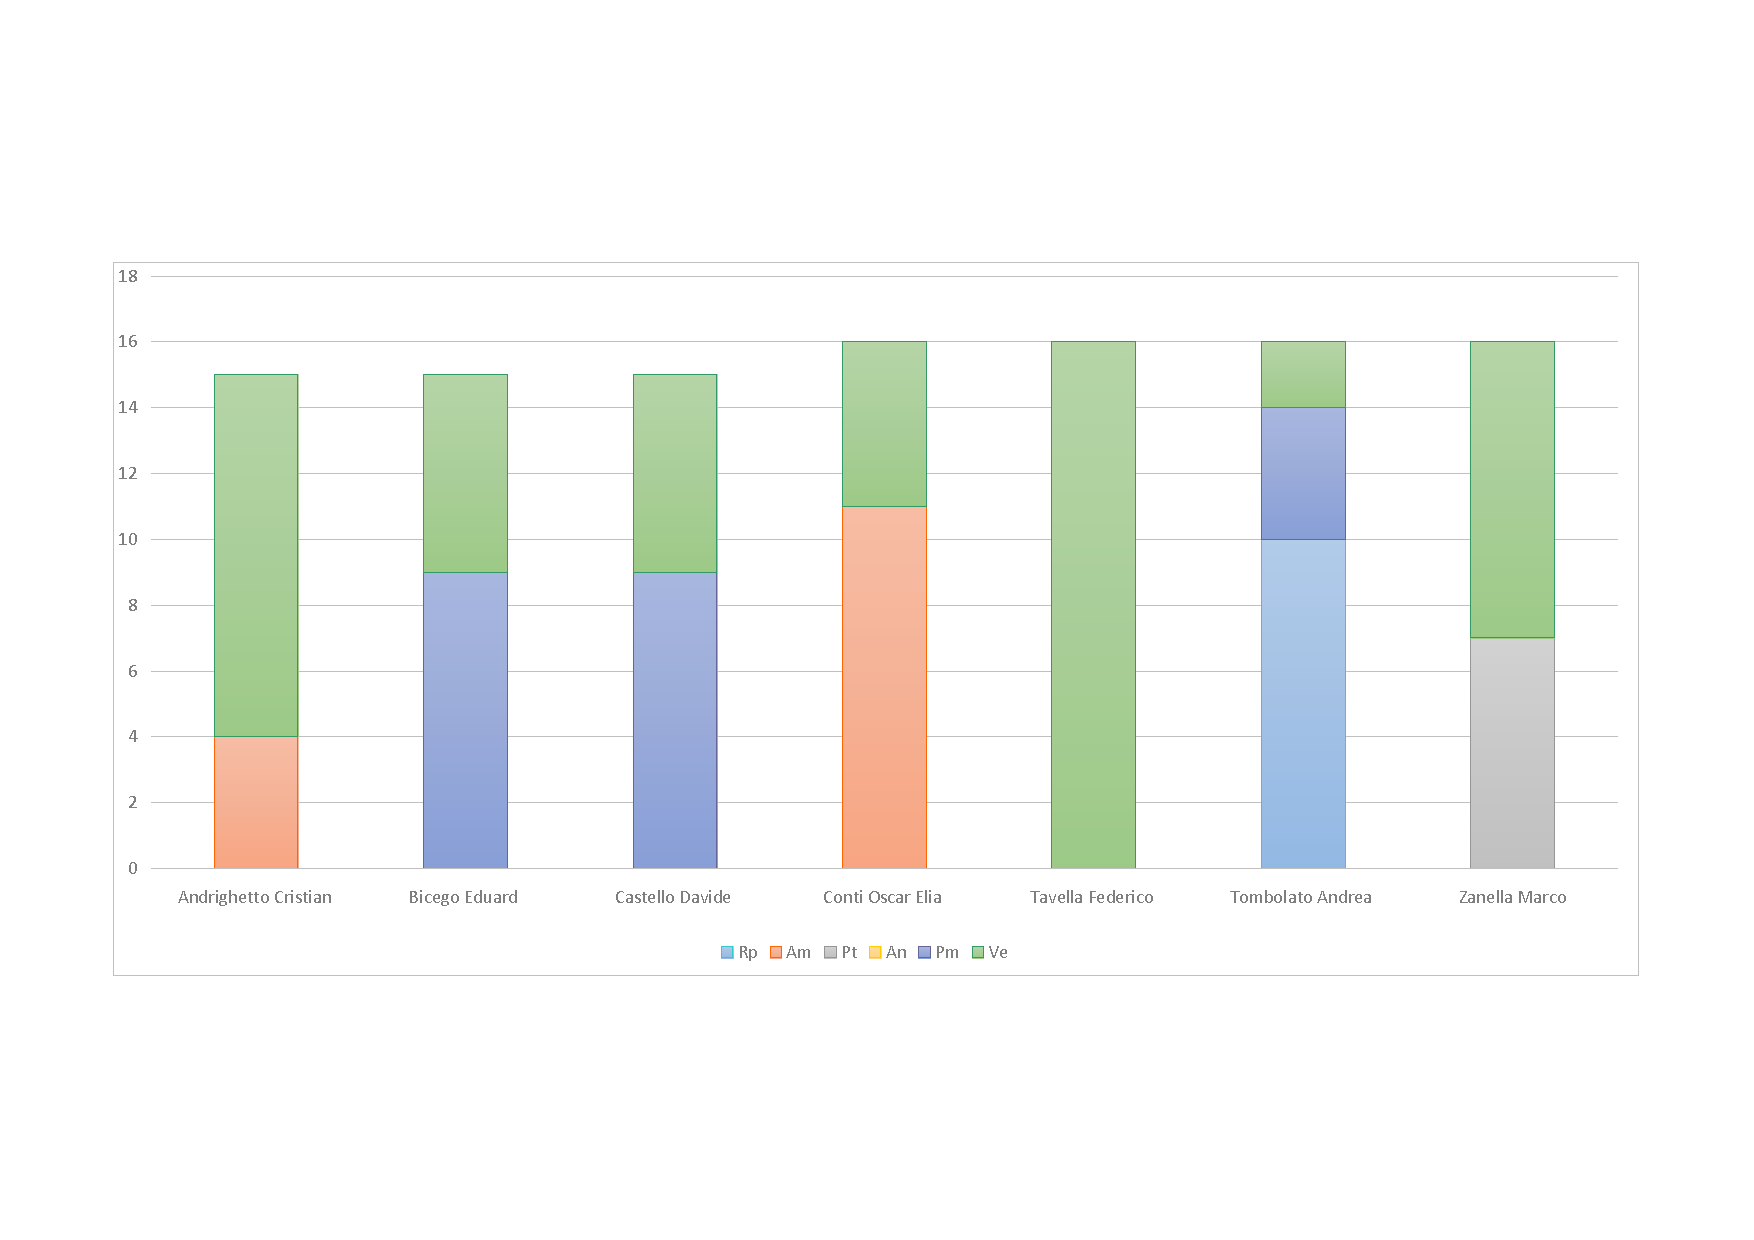
\includegraphics[width=\textwidth , trim=2cm 5cm 2cm 5cm]{grafici/V/V-ore-persona}
			\caption{Fase V - Riassunto}
		\label{fig:BarChart-faseV_ore}
	\end{figure}
\vfill	
\newpage
\vfill
	\paragraph{Prospetto economico}
					
	\begin{table}[h]
		\centering
	
		\begin{tabular}{l * {2}{c}}
			\toprule
			\textbf{Ruolo} & \textbf{Ore} & \textbf{Costo (\euro{})} \\
			\midrule
			Responsabile &	10 &  300,00 \\
			%\midrule
			Amministratore & 4 &  80,00 \\
			%\midrule
			Progettista & 7 & 154,00 \\
			%\midrule
			Analista & 0 & 0,00 \\
			%\midrule
			Programmatore & 24 & 370,00 \\
			%\midrule
			Verificatore & 55 & 825,00 \\
			\midrule		
			\textbf{Totale} & 100 & 1.719,00 \\
			\bottomrule	
		\end{tabular}
		\caption{Fase V - Costo per ruolo}
		\label{tab:faseV_costo}
	\end{table}
\vfill	
	
	\begin{figure}[!h]
		\centering
		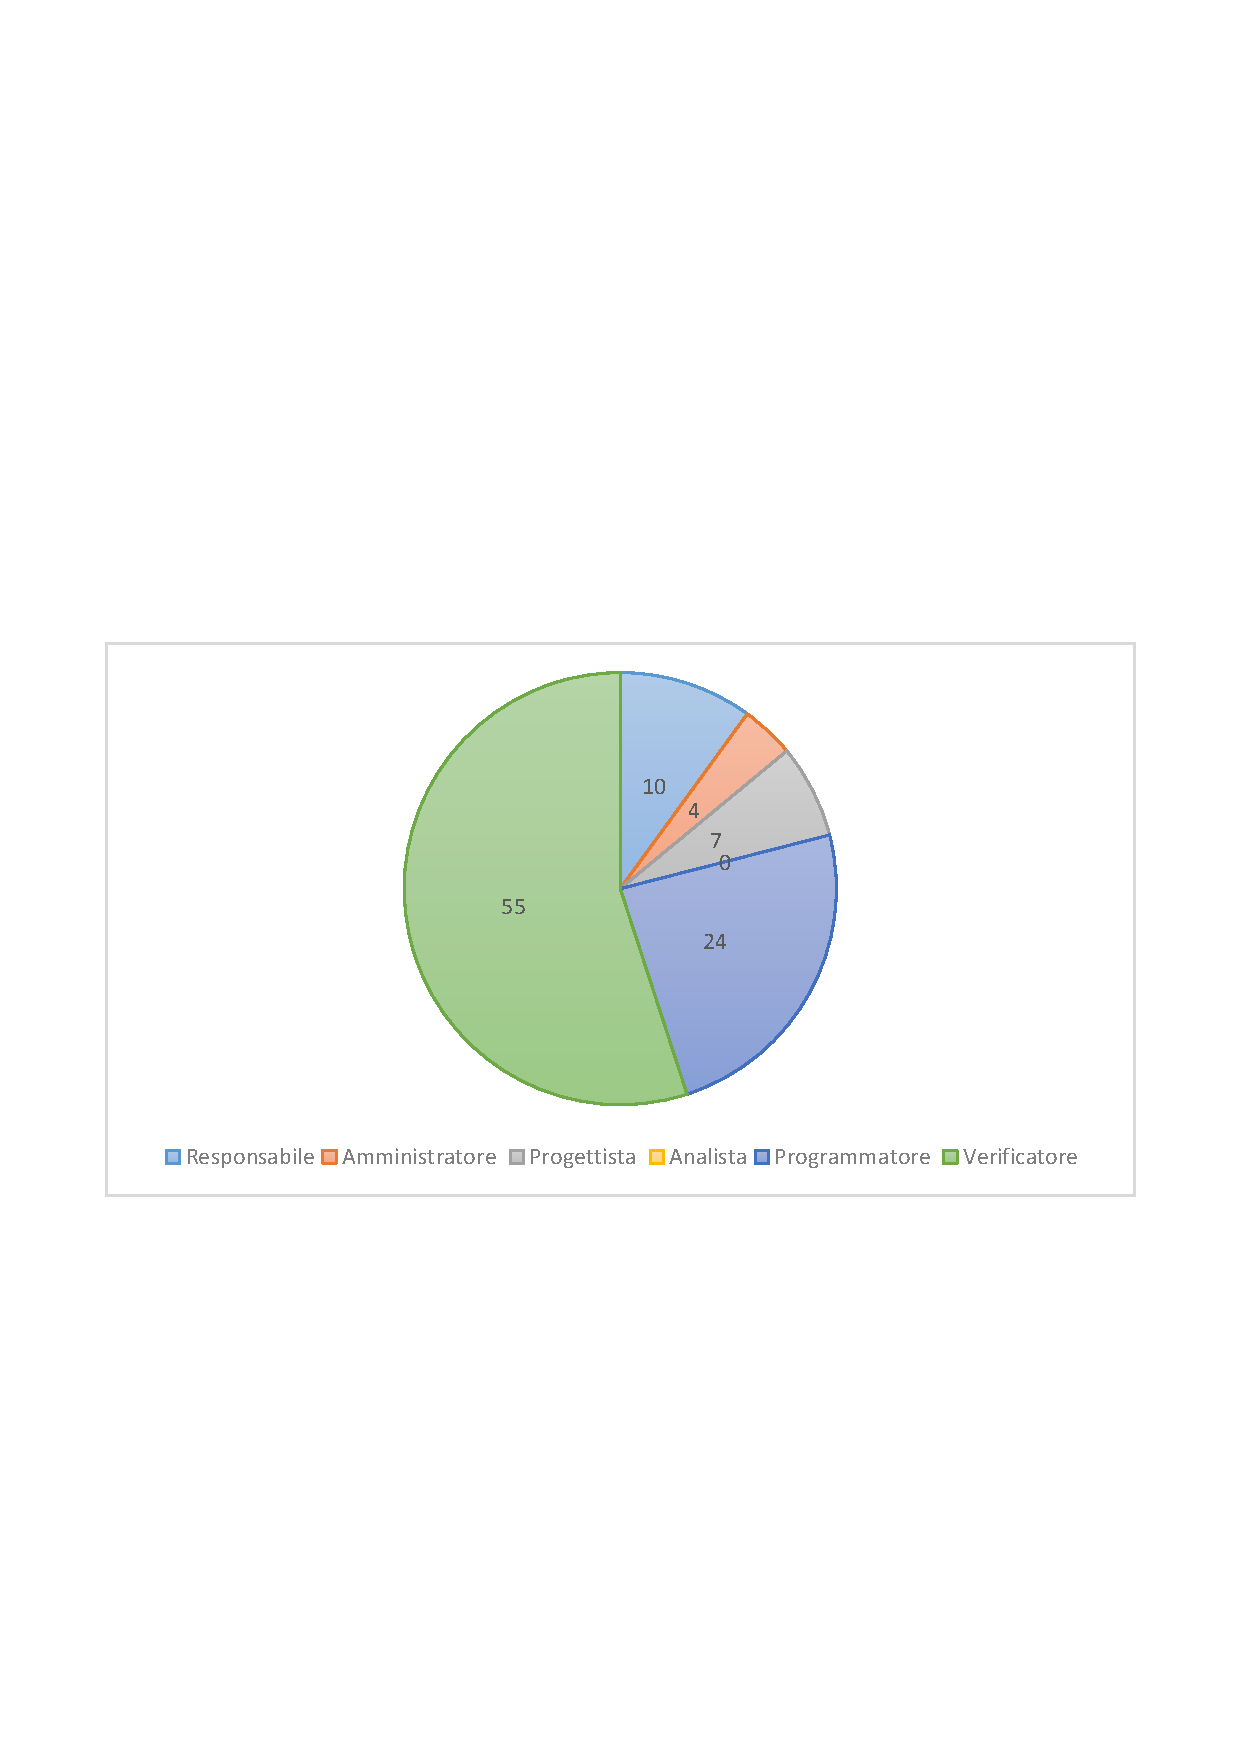
\includegraphics[width=0.93\textwidth , trim=2cm 9.5cm 2cm 11cm]{grafici/V/V-ore-ruolo}
			\caption{Fase V - Ore per ruolo}
		\label{fig:CircleChart-faseV_ore_r}
	\end{figure}
\vfill	
\newpage
	\begin{figure}[!h]
		\centering
		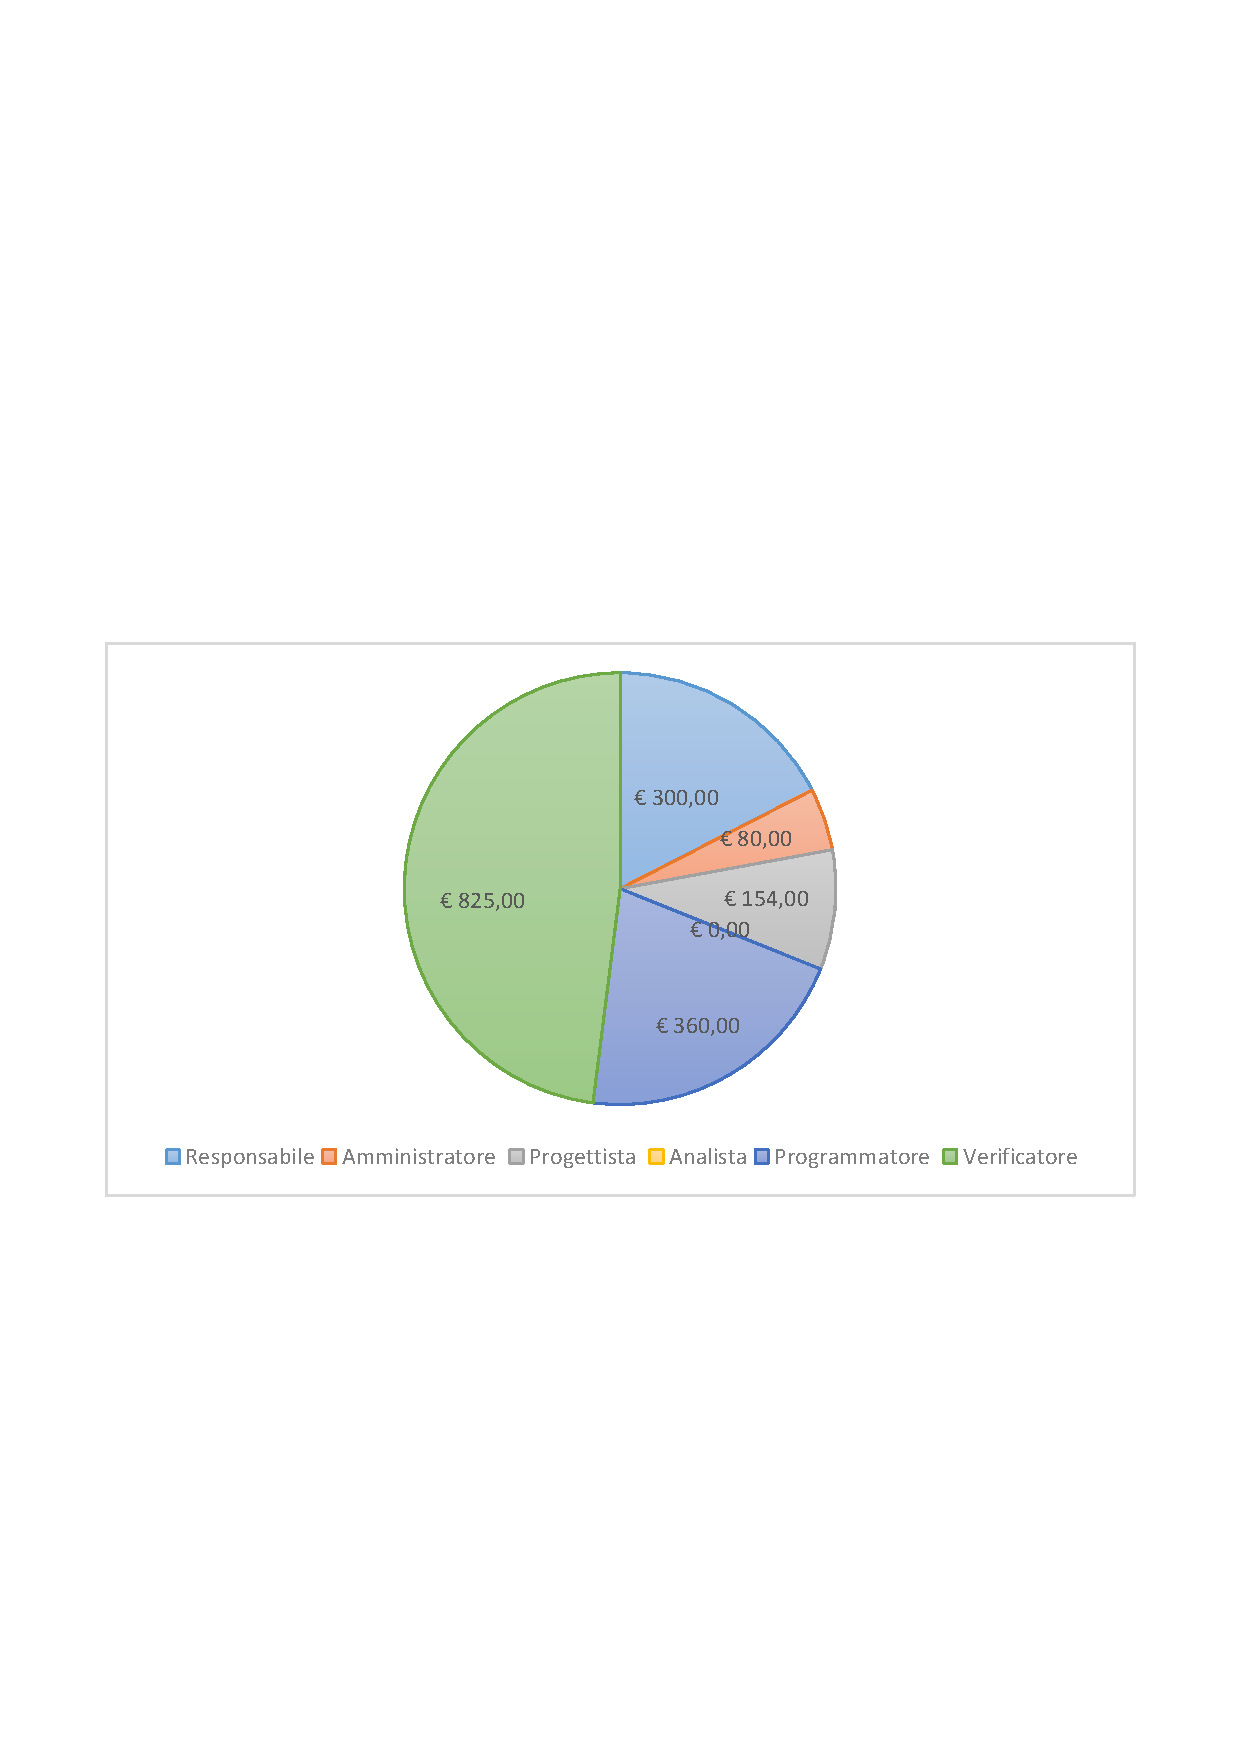
\includegraphics[width=0.93\textwidth , trim=2cm 9.5cm 2cm 11cm]{grafici/V/V-costo}
			\caption{Fase V - Costo per ruolo}
		\label{fig:CircleChart-faseV_costo}
	\end{figure}	
	
	\subsection{Riepilogo}
			\subsubsection{Ore totali}
				\paragraph{Suddivisione del lavoro}
					Le ore totali che ogni componente del gruppo \leaf\ dedicherà ad ognuno dei ruoli, a rotazione, sono indicate di seguito:
	
	\begin{table}[h]
		%\centering
		\begin{tabularx}{\textwidth}{l  * {6}{C}  c}
			\toprule
			\textbf{Nominativo} & \textbf{Rp} & \textbf{Am} & \textbf{Pt} 
						& \textbf{An} & \textbf{Pm} & \textbf{Ve} & \textbf{Ore totali} \\
			\midrule
			Andrighetto Cristian & 9 & 22 & 17 & 43 & 9 & 56 &	156 \\
			%\midrule
			Bicego Eduard & 9 & 20 & 23 & 30 & 27 & 46 & 155 \\
			%\midrule
			Castello Davide & 10 & 25 & 30 & 44 & 9 & 36 & 154 \\
			%\midrule
			Conti Oscar Elia & 17 & 24 & 36 & 22 & 15 & 36 & 150 \\
			%\midrule
			Tavella Federico &	17 & 9 & 26 & 26 & 18 & 46 & 142 \\
			%\midrule
			Tombolato Andrea & 22 & 10 & 43 & 26 & 21 & 35 & 157 \\
			%\midrule
			Zanella Marco & 20 & 22 & 33 & 27 & 12 & 37 & 151 \\
			\midrule			
			\textbf{Ore Totali Ruolo} & 104 & 132 & 208 & 218 & 111 & 292 & 1065 \\
			\bottomrule
		\end{tabularx}
		\caption{Ore totali - Suddivisione delle ore di lavoro}
		\label{tab:totale_ore}
	\end{table}
	
\newpage
\vfill
		
	\begin{figure}[!h]
		\centering
		\includegraphics[width=\textwidth , trim=2cm 5cm 2cm 5cm]{grafici/Riepilogo/Totali/ore-persona}
			\caption{Ore persona totali - Riassunto}
		\label{fig:BarChart-totale_ore}
	\end{figure}
	
\vfill	
	
	\paragraph{Prospetto economico}
					Il costo totale per ogni ruolo, comprensivo sia delle ore di formazione (a carico del gruppo \leaf) sia delle ore rendicontate (a carico del proponente), è dunque il seguente:
	\begin{table}[h]
		\centering
		\begin{tabular}{l * {2}{c}}
			\toprule
			\textbf{Ruolo} & \textbf{Ore} & \textbf{Costo (\euro{})} \\
			\midrule
			Responsabile &	104 & 3.120,00 \\
			%\midrule
			Amministratore & 132 & 2.640,00 \\
			%\midrule
			Progettista & 208 & 4.576,00 \\
			%\midrule
			Analista & 218 & 5.450,00 \\
			%\midrule
			Programmatore & 111 & 1.665,00 \\
			%\midrule
			Verificatore & 292 & 4.380,00 \\
			\midrule		
			\textbf{Totale} & 1065 &  21.831,00 \\
			\bottomrule
		\end{tabular}
		\caption{Ore totali - Costo per ruolo}
		\label{tab:totale_costo}
	\end{table}
\vfill
\newpage	
\vfill
	
	\begin{figure}[!h]
		\centering
		\includegraphics[width=0.93\textwidth , trim=2cm 9.5cm 2cm 11cm]{grafici/Riepilogo/Totali/ore-ruolo}
			\caption{Ore totali - Ore per ruolo}
		\label{fig:CircleChart-totale_ore_r}
	\end{figure}	
\vfill
	\begin{figure}[!h]
		\centering
		\includegraphics[width=0.93\textwidth , trim=2cm 9.5cm 2cm 11cm]{grafici/Riepilogo/Totali/costo}
			\caption{Ore totali - Costo per ruolo}
		\label{fig:CircleChart-totale_ore}
	\end{figure}
\vfill
\newpage
	
	\subsubsection{Ore di investimento}
				\paragraph{Suddivisione del lavoro}
					Le ore di investimento che ogni componente del gruppo \leaf\ dedicherà ad ognuno dei ruoli, a rotazione, vengono indicate di seguito:
	
	\begin{table}[h]
		%\centering
		\begin{tabularx}{\textwidth}{l  * {6}{C}  c}
			\toprule
			\textbf{Nominativo} & \textbf{Rp} & \textbf{Am} & \textbf{Pt} 
						& \textbf{An} & \textbf{Pm} & \textbf{Ve} & \textbf{Ore totali} \\
			\midrule
			Andrighetto Cristian & 5 & 15 & 5 & 13 &	0 &	9 &	47 \\
			%\midrule
			Bicego Eduard & 0 & 5 & 3 & 10 & 7 & 25 & 50 \\
			%\midrule
			Castello Davide & 5 & 15 & 5 & 18 & 0 & 9 & 52 \\
			%\midrule
			Conti Oscar Elia & 7 & 4 & 17 & 0 & 2 & 15 & 45 \\
			%\midrule
			Tavella Federico &	7 & 0 & 6 & 12 & 7 & 14 & 46 \\
			%\midrule
			Tombolato Andrea & 7 & 0 & 19 & 7 & 1 & 10 & 44 \\
			%\midrule
			Zanella Marco & 10 & 10 & 13 & 2 & 0 & 11 & 46 \\
			\midrule			
			\textbf{Ore Totali Ruolo} & 41 & 49 & 68 & 62 & 17 & 93 & 330 \\
			\bottomrule
		\end{tabularx}
		\caption{Ore di investimento - Suddivisione delle ore di lavoro}
		\label{tab:investimento_ore}
	\end{table}
\vfill	

	
	\begin{figure}[!h]
		\centering
		\includegraphics[width=\textwidth , trim=2cm 5cm 2cm 5cm]{grafici/Riepilogo/Investimento/ore-persona}
			\caption{Ore di investimento - Riassunto}
		\label{fig:BarChart-investimento_ore}
	\end{figure}
\vfill
\newpage
\vfill	
	\paragraph{Prospetto economico}
					Il costo d'investimento per ogni ruolo è dunque il seguente:
	\begin{table}[h]
		\centering
		\begin{tabular}{l * {2}{c}}
			\toprule
			\textbf{Ruolo} & \textbf{Ore} & \textbf{Costo (\euro{})} \\
			\midrule
			Responsabile &	41 &  1.230,00 \\
			%\midrule
			Amministratore & 29 & 980,00 \\
			%\midrule
			Progettista & 68 & 1.496,00 \\
			%\midrule
			Analista & 62 & 1.550,00 \\
			%\midrule
			Programmatore & 17 & 255,00 \\
			%\midrule
			Verificatore & 93 & 1.395,00 \\
			\midrule		
			\textbf{Totale} & 330 & 6.906,00 \\
			\bottomrule
		\end{tabular}
		\caption{Ore di investimento - Costo per ruolo}
		\label{tab:investimento_costo}
	\end{table}
\vfill	
	
	\begin{figure}[!h]
		\centering
		\includegraphics[width=0.93\textwidth , trim=2cm 9.5cm 2cm 11cm]{grafici/Riepilogo/Investimento/ore-ruolo}
			\caption{Ore di investimento - Ore per ruolo}
		\label{fig:CircleChart-investimento_ore_r}
	\end{figure}
\vfill	
\newpage
	\begin{figure}[!h]
		\centering
		\includegraphics[width=0.93\textwidth , trim=2cm 9.5cm 2cm 11cm]{grafici/Riepilogo/Investimento/costo}
			\caption{Ore di investimento - Costo per ruolo}
		\label{fig:CircleChart-investimento_costo}
	\end{figure}
\vfill	

	\subsubsection{Ore rendicontate}
				\paragraph{Suddivisione del lavoro}
					Le ore rendicontate che ogni componente del gruppo \leaf\ dedicherà ad ognuno dei ruoli, a rotazione, vengono indicate di seguito:
	
	\begin{table}[h]
		%\centering
		\begin{tabularx}{\textwidth}{l  * {6}{C}  c}
			\toprule
			\textbf{Nominativo} & \textbf{Rp} & \textbf{Am} & \textbf{Pt} 
						& \textbf{An} & \textbf{Pm} & \textbf{Ve} & \textbf{Ore totali} \\
			\midrule
			Andrighetto Cristian & 9 & 7 & 15 & 28 & 5 & 41 &	105 \\
			%\midrule
			Bicego Eduard & 9 & 15 & 20 & 20 & 20 & 21 & 105 \\
			%\midrule
			Castello Davide & 5 & 10 & 25 & 26 & 9 & 30 & 105 \\
			%\midrule
			Conti Oscar Elia & 10 & 20 & 19 & 22 & 13 & 21 & 105 \\
			%\midrule
			Tavella Federico &	10 & 9 & 20 & 16 & 15 & 35 & 105 \\
			%\midrule
			Tombolato Andrea & 10 & 10 & 21 & 19 & 20 & 25 & 105 \\
			%\midrule
			Zanella Marco & 10 & 12 & 20 & 25 & 12 & 26 & 105 \\
			\midrule			
			\textbf{Ore Totali Ruolo} & 63 & 83 & 140 & 156 & 94 & 199 & 735 \\
			\bottomrule
		\end{tabularx}
		\caption{Ore rendicontate - Suddivisione delle ore di lavoro}
		\label{tab:rendicontate_ore}
	\end{table}
	
\newpage
\vfill		
	
	\begin{figure}[!h]
		\centering
		\includegraphics[width=\textwidth , trim=2cm 5cm 2cm 5cm]{grafici/Riepilogo/Rendicontate/ore-persona}
			\caption{Ore rendicontate - Riassunto}
		\label{fig:BarChart-rendicontate_ore}
	\end{figure}
	
\vfill
	
	\paragraph{Prospetto economico}
					Il costo rendicontato per ogni ruolo è dunque il seguente:
	\begin{table}[h]
		\centering
		\begin{tabular}{l * {2}{c}}
			\toprule
			\textbf{Ruolo} & \textbf{Ore} & \textbf{Costo (\euro{})} \\
			\midrule
			Responsabile &	63 & 1.890,00 \\
			%\midrule
			Amministratore & 83 & 1.660,00 \\
			%\midrule
			Progettista & 140 & 3.080,00 \\
			%\midrule
			Analista & 156 & 3.900,00 \\
			%\midrule
			Programmatore & 94 & 1.410,00 \\
			%\midrule
			Verificatore & 199 & 2.950,00 \\
			\midrule		
			\textbf{Totale} & 735 & 14.925,00 \\
			\bottomrule
		\end{tabular}
		\caption{Ore rendicontate - Costo per ruolo}
		\label{tab:rendicontate_costo}
	\end{table}
\vfill
\newpage
\vfill	
	
	\begin{figure}[!h]
		\centering
		\includegraphics[width=0.93\textwidth , trim=2cm 9.5cm 2cm 11cm]{grafici/Riepilogo/Rendicontate/ore-ruolo}
			\caption{Ore rendicontate - Ore per ruolo}
		\label{fig:CircleChart-rendicontate_ore_r}
	\end{figure}
\vfill	
	\begin{figure}[!h]
		\centering
		\includegraphics[width=0.93\textwidth , trim=2cm 9.5cm 2cm 11cm]{grafici/Riepilogo/Rendicontate/costo}
			\caption{Ore rendicontate - Costo per ruolo}
		\label{fig:CircleChart-rendicontate_costo}
	\end{figure}
\vfill			
\end{document}